\documentclass{article}
\usepackage[paperwidth=210mm, paperheight=297mm, margin=2cm]{geometry}
%\usepackage[utf8]{inputenc}
%\usepackage{ebgaramond-maths}
\usepackage{ctex}
%==Math & Physics Packages==
\usepackage{amsmath, amsthm, amsfonts, amssymb}
\usepackage{mathrsfs}
\usepackage{setspace}
\usepackage{physics}
\usepackage{cancel}
\usepackage{nicefrac}
\usepackage{extarrows}

\usepackage{graphicx}
 \usepackage{booktabs}
\usepackage{longtable}
\usepackage{diagbox}


%==Image-related Packages==
\usepackage{graphics, graphicx}
\usepackage{tikz}
\usetikzlibrary{arrows.meta}
\usepackage{pgfplots}
\pgfplotsset{compat=1.18}
\usepackage{xcolor}
\usepackage{fourier-orns}
\usepackage{lipsum}
%==Colour Palette==
\definecolor{merah}{HTML}{F4564E}
\definecolor{merahtua}{HTML}{89313E}
\definecolor{biru}{HTML}{60BBE5}
\definecolor{birutua}{HTML}{412F66}
\definecolor{hijau}{HTML}{59CC78}
\definecolor{hijautua}{HTML}{366D5B}
\definecolor{kuning}{HTML}{FFD56B}
\definecolor{jingga}{HTML}{FBA15F}
\definecolor{ungu}{HTML}{8C5FBF}
\definecolor{lavender}{HTML}{CBA5E8}
\definecolor{merjamb}{HTML}{FFB6E0}

%==Theorems==
\usepackage{tcolorbox}
\tcbuselibrary{skins,breakable,theorems}
\usepackage{changepage}%用于调整页面布局,例如改变页面的宽度或高度。
\renewcommand{\thesection}{\arabic{section}.}

\makeatletter

        % Definition
%	\newtcbtheorem{dfn}{1}
%	{breakable,enhanced,arc=0mm,outer arc=0mm,
%		boxrule=0pt,toprule=1pt,leftrule=0pt,bottomrule=1pt, rightrule=0pt,left=0.2cm,right=0.2cm,
	%	titlerule=0.5em,toptitle=0.1cm,bottomtitle=-0.1cm,top=0.2cm,
	%	colframe=white!10!biru,colback=white!90!biru,coltitle=white,
     %       coltext=birutua!60!gray, title style={white!10!biru}, before skip=8pt, after skip=8pt,
		%fonttitle=\bfseries,fontupper=\normalsize}{dfn}
 
%==Formatting Packages==
\usepackage{multicol}
\usepackage{multirow}
\usepackage{enumitem}
\usepackage{indentfirst}
\usepackage[toc]{multitoc}

%==Layouting Packages==
\usepackage{titlesec}
\usepackage{fancyhdr}
\pagestyle{fancy}
\setlength{\headheight}{15pt}
% Uncomment jika perlu
\fancyhead[R]{xiaowen}
\fancyhead[L]{Coding and Information Theory}
%\fancyfoot[L]{}
\fancyfoot[C]{\thepage}
%\fancyfoot[R]{\thepage}






\renewcommand\headrule{%定义页眉中的水平线样式的
	\vspace{-6pt}%-1pt表示向上调整1个点的垂直间距
	\hrulefill
	\raisebox{-2pt}
	\hrulefill}

\renewcommand\footrule{%
	\hrulefill
	\raisebox{-2.1pt}
	%{\quad\floweroneleft\decoone\floweroneright\quad}%
	\hrulefill}
  
%Reference and Bibliography Packages==设置超链接的样式和颜色
\usepackage{hyperref}
\hypersetup{
    colorlinks=true,
    linkcolor={black},
    citecolor={biru!70!black},
    urlcolor={biru!80!black}
}

\numberwithin{equation}{section}%用于在 LaTeX 中设置公式编号的格式。具体来说,这行代码将使公式编号包含章节号,例如“1.1”表示第一章的第一个公式,以此类推。
%这行代码的作用是将公式编号设置为按节(section)进行编号,即每个节开始时公式编号会重新计数。这样可以更清晰地显示公式的编号,使其与章节结构相对应。

\begin{document}

\section{第一次课后作业}

\begin{tcolorbox}[breakable,colback=blue!5!white,colframe=blue!75!black,
 title= 单选题]
  概率分布 $ \bar{p}=\left\{p_{1}, p_{2}, \cdots, p_{a}\right\} $ 是一个确定性分布 为熵 $ H\left(p_{1}, p_{2}, \cdots, p_{a}\right)=0 $ 的(  ) 条件.

    
(A) 充分条件;
(B) 必要条件;
(C) 充分必要条件;
(D) 既不充分也不必要.
 \tcblower

概率分布 $\bar{p}=\left\{p_{1}, p_{2}, \cdots, p_{a}\right\}$ 是一个确定性分布,即所有的概率都为1或0,因此熵 $H\left(p_{1}, p_{2}, \cdots, p_{a}\right)=0$.

反之,若$H\left(p_{1}, p_{2}, \cdots, p_{a}\right)=0 \text {, 则由 } H\left(p_{1}, p_{2}, \cdots, p_{a}\right) \text { 的 }
$
定义可知, $ \forall i, p_{i} \log _{c} p_{i}=0 $, 或者 $ p_{i}=0 $, 或者 $ \log _{c} p_{i}=0 $, 由于 $ \sum\limits_{i=1}^{a} p_{i}=1, p_{i} \geq 0 $, 存在 $ i $ 使得 $ p_{i}=1 $, 而其它 $ p_{j}=0 $, 因此 $ \bar{p} $ 必为确定型分布.

所以,答案是:(C) 充分必要条件


\end{tcolorbox}


\begin{tcolorbox}[breakable,colback=blue!5!white,colframe=blue!75!black,
 title= 单选题]
 设 $ \xi $ 是一个二元随机变量, 即 $ \mathscr{X}=\{0,1\} $,令 $ p(\xi=1)=p, p(\xi=0)=1-p $. 则有二元熵函数 $ H(p)=p \log _{2} \frac{1}{p}+(1-p) \log _{2} \frac{1}{1-p} $,则当 $ p=$(  ) 时, $ H(p) $ 达到最大值.

(A) $ 0  $ (B) $ \frac{1}{4} $;
(C) $ \frac{1}{2} $;(D) 1 .
  \tcblower
  首先,计算 $ H(p) $ 的导数:
$$
\begin{aligned}
H(p) & =-p \log_2 p-(1-p) \log_2 (1-p) \\
H^{\prime}(p) & =-\log_2 p-p \cdot \frac{1}{\ln 2 \cdot p}+\log_2 (1-p)+\frac{1}{1-p} \cdot \frac{1-p}{\ln 2} \\
& =-\log_2 p-\frac{1}{\ln 2}+\log_2 (1-p)+\frac{1}{\ln 2} \\
& =-\log_2 p+\log_2 (1-p) \\
& =\log_2 \frac{1-p}{p}
\end{aligned}
$$
令导数等于零,解方程 $ \log _{2} \frac{1-p}{p}=0 $,得到 $ p=\frac{1}{2} $.

接下来,我们来验证 $ p=\frac{1}{2} $ 是 $ H(p) $ 的最大值点还是最小值点.我们可以通过二阶导数的符号来判断.计算二阶导数:
$$
\begin{aligned}
\frac{d^{2} H(p)}{d p^{2}} &=\frac{d}{d p}\left[\log _{2} \frac{1-p}{p}\right] \\
&=\frac{1}{p(p-1)\ln 2}
\end{aligned}
$$
当 $ p=\frac{1}{2} $ 时,$ \frac{1}{p(p-1)\ln 2}<0 $,所以 $ p=\frac{1}{2} $ 是 $ H(p) $ 的最大值点.

因此,当 $ p=\frac{1}{2} $ 时,$ H(p) $ 达到最大值.选项 (C) $ \frac{1}{2} $ 是正确答案.
\end{tcolorbox}

\begin{tcolorbox}[breakable,colback=blue!5!white,colframe=blue!75!black,
 title= 单选题]
若 $ H(\xi, \eta)=H(\xi)+H(\eta) $ ,则随机变量 $ \xi $与 $\eta$ 的关系(  ).

A. $ \xi $ 由 $ \eta $ 决定;

B. $ \eta $ 由$ \xi $决定;

C. $ \xi $ 与 $ \eta $ 相互独立.

  \tcblower

当两个随机变量 $\xi$ 和 $\eta$ 相互独立时,它们的联合概率分布可以表示为它们各自的边缘概率分布的乘积,即 $p(\xi, \eta) = p(\xi) \cdot p(\eta)$.根据熵的定义,随机变量的熵可以表示为 $H(\xi) = -\sum\limits_{{X}} p(x) \log p(x)$,其中 $x$ 是随机变量 $\xi$ 的取值.同样地,$H(\eta) = -\sum\limits_{{Y}} p(y) \log p(y)$,其中 $y$ 是随机变量 $\eta$ 的取值.当两个随机变量相互独立时,它们的联合熵可以表示为 $H(\xi, \eta) = -\sum\limits_{X}\sum\limits_{Y} p(x, y) \log p(x, y)$.由于它们相互独立,联合概率分布可以拆分为各自的边缘概率分布的乘积,即 $p(x, y) = p(x) \cdot p(y)$.代入联合熵的定义中,我们有:

$$
\begin{aligned}
H(\xi, \eta) &= -\sum_{X}\sum_{Y} p(x, y) \log p(x, y) \\
&= -\sum_{{X}}\sum_{Y} p(x) \cdot p(y) \log (p(x) \cdot p(y)) \\
&= -\sum_{X}\sum_{Y} p(x) \cdot p(y) (\log p(x) + \log p(y)) \\
&= -\sum_{X}\sum_{Y} p(x) \cdot p(y) \log p(x) - \sum_{X}\sum_{Y} p(x) \cdot p(y) \log p(y) \\
&= -\sum_{X} p(x) \log p(x) - \sum_{Y} p(y) \log p(y) \\
&= H(\xi) + H(\eta)
\end{aligned}
$$

因此,当 $H(\xi, \eta) = H(\xi) + H(\eta)$ 时,可以得出 $\xi$ 和 $\eta$ 是相互独立的.

\end{tcolorbox}



\begin{tcolorbox}[breakable,colback=blue!5!white,colframe=blue!75!black,
 title= 单选题]
$  \mathrm{H}(\xi, \eta)=\mathrm{H}(\xi) $ ,则随机变量 $ \xi $ 与 $ \eta $ 的关系 ( ).

A. $ \xi $ 由 $ \eta $ 决定;

B. $ \xi $ 与相互独立;

C. $ \eta $ 由$ \xi $决定.
  \tcblower

根据题目中的信息 $ \mathrm{H}(\xi, \eta)=\mathrm{H}(\xi) $,这意味着给定 $ \xi $ 的情况下, $ \eta $ 的条件熵为零,即 $ \mathrm{H}(\eta|\xi) = 0 $.这表明在已知 $ \xi $ 的情况下, $ \eta $ 是确定的,因此可以得出结论: $ \eta $ 由 $ \xi $ 决定.因此,答案是 C. $ \eta $ 由 $ \xi $ 决定.

\end{tcolorbox}


\begin{tcolorbox}[breakable,colback=blue!5!white,colframe=blue!75!black,
 title=计算题]
计算 $ H\left(\frac{1}{a}, \frac{1}{a}, \cdots, \frac{1}{a}, \frac{2}{a}, \frac{2}{a}\right) $


 \tcblower
由 $ \Sigma P_{i}=1 $ 知,含 $ (a-4) $ 个 $ \frac{1}{a}$ , 2 个$ \frac{2}{a} $ ,总共$ (a-2) $ 项, 于是
$$
\begin{aligned}
H\left(\frac{1}{a}, \frac{1}{a}, \cdots, \frac{1}{a}, \frac{2}{a}, \frac{2}{a}\right) & =\sum_{i=1}^{a-2} p_{i} \cdot \log \frac{1}{p_{i}} \\
& =\sum_{i=1}^{a-4} \frac{1}{a} \log a+2 \cdot \frac{2}{a} \log \frac{a}{2} \\
& =\frac{a-4}{a} \cdot \log a+\frac{4}{a} \log \frac{a}{2} \\
& =\frac{a-4}{a} \cdot \log a+\frac{4}{a} \log a-\frac{4}{a} \log 2 \\
& =\log a-\frac{4}{a} \log 2
\end{aligned}
$$
\end{tcolorbox}


\begin{tcolorbox}[breakable,colback=blue!5!white,colframe=blue!75!black,
 title=计算题]
设两只口袋中各有20个球,第一支口袋中有10个白球,5个黑球和5 个红球; 第二只口袋中有8个白球, 8 个黑球和 4 个红球,从每只口袋中各取一个球, 试判断哪一个结果的不肯定性更大.


 \tcblower
当我们要判断哪个结果的不确定性更大时,可以使用熵来衡量.
首先,我们将第一只口袋的球的颜色作为随机变量 $\xi_1$,它的概率分布为:
$$
\xi_1 \sim \left(\begin{array}{ccc}\text{白} & \text{黑} & \text{红} \\ \frac{1}{2} & \frac{1}{4} & \frac{1}{4}\end{array}\right)
$$
其中,$\frac{1}{2}$ 表示白球的概率,$\frac{1}{4}$ 表示黑球的概率,$\frac{1}{4}$ 表示红球的概率.

计算第一只口袋的熵 $H(\xi_1)$:
$$ H\left(\xi_{1}\right)=\frac{1}{2} \log 2+2 \times \frac{1}{4} \log 4=\frac{1}{2}+1=1.5  \text{ bits}
$$
接下来,我们将第二只口袋的球的颜色作为随机变量 $\xi_2$,它的概率分布为:
$$
\xi_2 \sim \left(\begin{array}{ccc}\text{白} & \text{黑} & \text{红} \\ \frac{2}{5} & \frac{2}{5} & \frac{1}{5}\end{array}\right)
$$
其中,$\frac{2}{5}$ 表示白球的概率,$\frac{2}{5}$ 表示黑球的概率,$\frac{1}{5}$ 表示红球的概率.

计算第二只口袋的熵 $H(\xi_2)$:

$$
\begin{aligned}
H\left(\xi_{2}\right) & =\frac{4}{5} \log \frac{5}{2}+\frac{1}{5} \log 5 \\
& =\frac{4}{5}(\log 5-\log 2)+\frac{1}{5} \log 5 \\
& =\frac{4}{5} \log 5+\frac{1}{5} \log 5-\frac{4}{5} \\
& =\log 5-\frac{4}{5} \approx 2.32-0.8 \\
& =1.52 \text { bits }
\end{aligned}
$$
比较 $H(\xi_1)$ 和 $H(\xi_2)$ 的值,我们可以得出结论:第二只口袋的结果的不确定性更大,因为它的熵值更大. 
\end{tcolorbox}




\section{第二次课后作业}

\begin{tcolorbox}[breakable,colback=blue!5!white,colframe=blue!75!black,
 title= 单选题]
 互信息 $ I(\xi; \eta)=0 $ 的充分必要条件是随机变量 $ \xi $ 与 $ \eta $ 的关系为 ( ).

A. $ \eta $ 由 $ \xi $ 决定

B.  相互独立

C.  $ \xi $ 由 $ \eta $ 决定

\tcblower
根据互信息与联合熵的关系可知,$ I(\xi, \eta) =H(\xi)+H(\eta)-H(\xi,\eta)=0 $,于是我们有$ H(\xi)+H(\eta)=H(\xi,\eta) $.由前面知$ \eta $ 与$ \xi $相互独立.
因此,互信息为零是 $ \xi $ 和 $ \eta $ 相互独立的充分必要条件.

\end{tcolorbox}

\begin{tcolorbox}[breakable,colback=blue!5!white,colframe=blue!75!black,
 title= 填空题]
 令 $ \xi $ 是一个离散随机变量,它服从的概率分布是 $ \overline{p}=\left(p_{1}, p_{2}, \cdots p_{a}\right) $, 则 $ \xi $ 的熵 $ {H}(\xi)=\underline{\hspace{1cm}} $ ,它在$\underline{\hspace{1cm}}$ 条件下达到最大值,最大值 $ = \underline{\hspace{1cm}}$.

\tcblower

对于离散随机变量 $ \xi $,其熵 $ H(\xi) $ 定义为:

$$ H(\xi) = -\sum_{i=1}^{a} p_i \log p_i $$

其中,$ p_i $ 是 $ \xi $ 取第 $ i $ 个值的概率,$ a $ 是 $ \xi $ 可能取的值的个数.

当 $ \xi $ 的概率分布是均匀分布时,即所有可能取值的概率相等,即 $ p_i = \frac{1}{a} $,此时熵 $ H(\xi) $ 达到最大值.在这种情况下,熵的最大值为:

$$ H_{\text{max}} = -\sum_{i=1}^{a} \frac{1}{a} \log \frac{1}{a} = -a \cdot \frac{1}{a} \log \frac{1}{a} = \log a $$

因此,当 $ \xi $ 的概率分布是均匀分布时,熵 $ H(\xi) $ 达到最大值,最大值为 $ \log a $.

\end{tcolorbox}



\begin{tcolorbox}[breakable,colback=blue!5!white,colframe=blue!75!black,
 title= 填空题]
 设$p(x)$ ,$q(x)$是离散信源$\mathscr{X}$上的两个概率分布,则它们的互熵$H(p||q)=0$的充分必要条件是 $\underline{\hspace{1cm}}$ .
\tcblower
当 $ H(p||q) = 0 $ 时,根据互熵的定义,我们有:
$$
\begin{aligned}
H(p \| q) & =\sum_{x \in \mathscr{X}} p(x) \log \frac{p(x)}{q(x)}=\sum_{x \in \mathscr{X}} p(x) [\log p(x) - \log q(x)]=0\\
\end{aligned}
$$
因此, 当且仅当对任意$q(x)\neq 0$的 $ x $, 满足 $ p(x)=q(x)$时$ H(p \| q)=0 $ .



\end{tcolorbox}


\begin{tcolorbox}[breakable,colback=blue!5!white,colframe=blue!75!black,
 title= 填空题]
 互信息$I(\xi;\eta)$与熵$H(\xi)$,$H(\eta)$及联合熵$H(\xi,\eta)$满足关系式$\underline{\hspace{2cm}}$ .

\tcblower
$$
 \begin{aligned}
& I(\xi ; \eta)=\sum_{x \in \mathscr{X}} \sum_{y \in \mathscr{Y}} p(x, y) \log \frac{p(x, y)}{p(x) q(y)} \\
= & \sum_{x \in \mathscr{X}} \sum_{y \in \mathscr{Y}} p(x, y)[\log p(x, y)-\log p(x) q(y)] \\
= & \sum_{x \in \mathscr{X}} \sum_{y \in \mathscr{Y}} p(x, y)[\log p(x, y)-\log p(x)-\log q(y)] \\
= & \sum_{x \in \mathscr{X}} \sum_{y \in \mathscr{Y}} p(x, y) \log p(x, y)-\sum_{x \in \mathscr{X}} \sum_{y \in \mathscr{Y}} p(x, y) \log p(x)  -\sum_{x \in \mathscr{X}} \sum_{y \in \mathscr{Y}} p(x, y) \log q(y) \\
= & -H(\xi, \eta)+H(\xi)+H(\eta)=H(\xi)+H(\eta)-H(\xi, \eta)
\end{aligned}
$$
即$ I(\xi; \eta) =H(\xi)+H(\eta)-H(\xi,\eta) $.
\end{tcolorbox}


\begin{tcolorbox}[breakable,colback=blue!5!white,colframe=blue!75!black,
 title= 解答题]
 令 $ (\xi, \eta) $ 具有如下联合分布
\begin{tabular}{|c|cccc|}
\hline\diagbox{$ \eta $}{$ \xi $} & 1 & 2 & 3 & 4 \\
\hline 1 & $ \frac{1}{8} $ & $ \frac{1}{16} $ & $ \frac{1}{32} $ & $ \frac{1}{32} $ \\
2 & $ \frac{1}{16} $ & $ \frac{1}{8} $ & $ \frac{1}{32} $ & $ \frac{1}{32} $ \\
3 & $ \frac{1}{8} $ & $ \frac{1}{8} $ & 0 & 0 \\
4 & $ \frac{1}{16} $ & $ \frac{1}{16} $ & $ \frac{1}{16} $ & $ \frac{1}{16} $ \\
\hline
\end{tabular}

试求:(1) $ H(\xi), H(\eta) $; (2) $ H(\xi \mid \eta), H(\eta \mid \xi) $; (3) $ H(\xi, \eta) $;
(4) $ H(\eta)-H(\eta \mid \xi) $; (5) $ I(\xi ; \eta) $.

\tcblower

\begin{center}
\begin{tabular}{|c|cccc|c|}
\hline
\diagbox{$ \eta $}{$ \xi $}
 & $1$ & $2$ & $3$ & $4$ & $ \sum $ \\
\hline $1$ & $ \frac{1}{8} $ & $ \frac{1}{16} $ & $ \frac{1}{32} $ & $ \frac{1}{32} $ & $ \frac{1}{4} $ \\
$2$ & $ \frac{1}{16} $ & $ \frac{1}{8} $ & $ \frac{1}{32} $ & $ \frac{1}{32} $ & $ \frac{1}{4} $ \\
$3$ & $ \frac{1}{8} $ & $ \frac{1}{8} $ & $ 0 $ & $ 0 $ & $ \frac{1}{4} $ \\
$4$ & $ \frac{1}{16} $ & $ \frac{1}{16}$ & $ \frac{1}{16}$ & $ \frac{1}{16}$ & $ \frac{1}{4} $ \\
\hline $\sum$ & $\frac{3}{8}$ & $\frac{3}{8}$ & $\frac{1}{8}$ & $\frac{1}{8}$ & $1 $ \\
\hline
\end{tabular}
\end{center}
对  $\xi: p(x)=\sum\limits_{y \in \mathscr{Y}} p(x, y)$, 则有:
$$
\begin{array}{l} 
p(1)=p(1,1)+p(1,2)+p(1,3)+p(1,4) 
=\frac{1}{8}+\frac{1}{16}+\frac{1}{8}+\frac{3}{8}=\frac{3}{8} \\
p(2)=p(2,1)+p(2,2)+p(2,3)+p(2,4) 
=\frac{1}{16}+\frac{1}{8}+\frac{1}{8}+\frac{1}{16}=\frac{3}{8} \\
p(3)=p(3,1)+p(3,2)+p(3,3)+p(3,4) 
=\frac{1}{32}+\frac{1}{32}+0+\frac{1}{16}=\frac{1}{8} \\
p(4)=p(4,1)+p(4,2)+p(4,3)+p(4,4) 
=\frac{1}{32}+\frac{1}{32}+0+\frac{1}{16}=\frac{1}{8}
\end{array}
$$
因此 $ \xi $ 的边缘分布为 $ \left(\frac{3}{8}, \frac{3}{8}, \frac{1}{8}, \frac{1}{8}\right) $ .同理对 $\eta: p(y)=\sum\limits_{x \in \mathscr{X}} p(x, y)$,
也可求得$\eta$的边缘分布为 $ \left(\frac{1}{4}, \frac{1}{4} , \frac{1}{4}, \frac{1}{4}\right) $.于是
$$\begin{aligned}
     H(\xi)&=\sum_{i=1}^{4} p_{i} \log \frac{1}{p_{i}}=2 \cdot \frac{3}{8} \cdot \log _{2} \frac{8}{3}+2 \cdot \frac{1}{8} \cdot \log _{2} 8 =3-\frac{3}{4} \log _{2} 3 \\
H(\eta)&=\sum_{i=1}^{4} p_{i} \log \frac{1}{p_{i}}=4 \cdot \frac{1}{4} \log _{2} 4=2 \\
H(\xi, \eta)&=\sum_{x \in \mathscr{X}} \sum_{y \in \mathscr{Y}} p(x, y) \cdot \log _{2} \frac{1}{p(x, y)} 
=4 \cdot \frac{1}{8} \cdot \log _{2} 8+6 \cdot \frac{1}{16} \cdot \log _{2} 16+4 \cdot \frac{1}{32} \log _{2} 32 \\
&=\frac{3}{2}+\frac{3}{2}+\frac{5}{8}=\frac{29}{8} 
\end{aligned}$$
$$
\begin{array}{l}
H(\xi \mid \eta)=H(\xi, \eta)-H(\eta)=\frac{29}{8}-2=\frac{13}{8} \\
H(\eta \mid \xi)=H(\xi, \eta)-H(\xi)=\frac{29}{8}-\left(3-\frac{3}{4} \log _{2} 3\right)=\frac{5}{8}+\frac{3}{4} \log _{2} 3 \\
H(\eta)-H(\eta \mid \xi)=2-\left(\frac{5}{8}+\frac{3}{4} \log _{2} 3\right)=\frac{11}{8}-\frac{3}{4} \log _{2} 3 \\
I(\xi ; \eta)=H(\xi)+H(\eta)-H(\xi, \eta) =3-\frac{3}{4} \log _{2} 3+2-\frac{29}{8} =\frac{11}{8}-\frac{3}{4} \log _{2} 3 
\end{array}
$$

\end{tcolorbox}


\begin{tcolorbox}[breakable,colback=blue!5!white,colframe=blue!75!black,
 title= 解答题]
 设两只口袋中各有20个球,第一支口袋中有10个白球,5个黑球和5个红球; 第二只口袋中有8个白球,6个黑球和6 个红球,从每只口袋中各取一个球,试判断哪一个结果的不肯定性更大(已知: $ \log _{2} 5=2.322, \log _{2} 3=1.585 $ ).
\tcblower

当我们要判断哪个结果的不肯定性更大时,可以使用熵来衡量.
首先,我们将第一只口袋的球的颜色作为随机变量 $\xi_1$,它的概率分布为:
$$
\xi_1 \sim \left(\begin{array}{ccc}\text{白} & \text{黑} & \text{红} \\ \frac{1}{2} & \frac{1}{4} & \frac{1}{4}\end{array}\right)
$$
其中,$\frac{1}{2}$ 表示白球的概率,$\frac{1}{4}$ 表示黑球的概率,$\frac{1}{4}$ 表示红球的概率.

计算第一只口袋的熵 $H(\xi_1)$:
$$ H\left(\xi_{1}\right)=\frac{1}{2} \log _{2} 2+\frac{1}{4} \log _{2} 4+\frac{1}{4} \cdot \log _{2} 4 \\ =\frac{1}{2}+\frac{1}{2}+\frac{1}{2}=1.5  \text{ bits}
$$
接下来,我们将第二只口袋的球的颜色作为随机变量 $\xi_2$,它的概率分布为:
$$
\xi_2 \sim \left(\begin{array}{ccc}\text{白} & \text{黑} & \text{红} \\ \frac{2}{5} & \frac{3}{10} & \frac{3}{10}\end{array}\right)
$$
其中,$\frac{2}{5}$ 表示白球的概率,$\frac{3}{10}$ 表示黑球的概率,$\frac{3}{10}$ 表示红球的概率.

计算第二只口袋的熵 $H(\xi_2)$:

$$
\begin{aligned}
H\left(\xi_{2}\right) & =\frac{2}{5} \log _{2} \frac{5}{2}+\frac{3}{10} \log _{2} \frac{10}{3}+\frac{3}{10} \log _{2} \frac{10}{3} \\
&=\frac{2}{5}\left(\log _{2} 5-1\right)+\frac{3}{5}\left(\log _{2} 10-\log _{2} 3\right) \\
&=\frac{2}{5}\left(\log _{2} 5-1\right)+\frac{3}{5}\left(1+\log _{2} 5-\log _{2} 3\right) \\
&  =\log _{2} 5-\frac{3}{5} \log _{2} 3+\frac{1}{5} \\
& \approx 2.322-0.6\times 1.585+0.2\\
& =1.571 \text { bits }
\end{aligned}
$$

所以我们得到$H(\xi_1)=1.5<1.571=H(\xi_2)$,
比较 $H(\xi_1)$ 和 $H(\xi_2)$ 的值,我们可以得出结论:第二只口袋的结果的不肯定性更大,因为它的熵值更大. 



\end{tcolorbox}




\section{第三次课后作业}

\begin{tcolorbox}[breakable,colback=blue!5!white,colframe=blue!75!black,
 title= 2024-03-11]
 设 $ \xi $ 和 $ \eta $ 联合分布 $ p(0,0)=\frac{1}{3}, p(0,1)=\frac{1}{3}, p(1,0)=0 $, $ p(1,1)=\frac{1}{3} $, 试求:
 
(1) $ H(\xi), H(\eta) $;

(2) $ H(\xi \mid \eta), H(\eta \mid \xi) $;

(3) $ H(\xi, \eta) $;

(4) $ H(\eta)-H(\eta \mid \xi) $;

(5) $ I(\xi ; \eta) $;

(6) 画出上述各信息之间关系的韦恩图.

\tcblower
\begin{center}
     \begin{tabular}{|c|cc|c|}
\hline\diagbox{$ \eta $}{$ \xi $} & 0 & 1 & $ \sum $ \\
\hline 0 & $ \frac{1}{3} $ & 0 & $ \frac{1}{3} $ \\
\hline 1 & $ \frac{1}{3} $ & $ \frac{1}{3} $ & $ \frac{2}{3} $ \\
\hline$ \sum $ & $ \frac{2}{3} $ & $ \frac{1}{3} $ & 1 \\
\hline
\end{tabular}$\quad\Longrightarrow$
$
\xi \sim\left(\begin{array}{cc}
0 & 1 \\
\frac{2}{3} & \frac{1}{3}
\end{array}\right), \quad \eta \sim\left(\begin{array}{cc}
0 & 1 \\
\frac{1}{3} & \frac{2}{3}
\end{array}\right)
$
\end{center}
(1)
$$
\begin{aligned}
H(\xi)  =\sum_{i=0}^{1} p_{i} \log_2 \frac{1}{p_{i}}=\frac{2}{3} \log_2 \frac{3}{2}+\frac{1}{3} \log_2 3 =\frac{2}{3} \log_ 3-\frac{2}{3} \log_ 2+\frac{1}{3} \log_2 3  =\log_2 3-\frac{2}{3}
\end{aligned}
$$
$$
\begin{aligned}
H(\eta)  =\sum_{i=0}^{1} p_{i} \log_2 \frac{1}{p_{i}}=\frac{1}{3} \log_2 3+\frac{2}{3} \log_2 \frac{3}{2}  =\frac{1}{3} \log_2 3+\frac{2}{3} \log_2 3-\frac{2}{3} \log_2 2 \ =\log_2 3-\frac{2}{3}
\end{aligned}
$$
(3)
$$
\begin{aligned}
H(\xi, \eta) & =\sum_{x \in \mathscr{X}} \sum_{x \in \mathscr{Y}} p(x, y) \log \frac{1}{p(x, y)}  =3 \cdot \frac{1}{3} \log_2 3=\log_2 3
\end{aligned}
$$
(2)
$$
\begin{aligned}
H(\eta \mid \xi) & =H(\xi, \eta)-H(\xi)  =\log_2 3-\left(\log_2 3-\frac{2}{3}\right)=\frac{2}{3} \\
H(\xi \mid \eta) & =H(\xi, \eta)-H(\eta)  =\log_2 3-\left(\log_2 3-\frac{2}{3}\right)=\frac{2}{3}
\end{aligned}
$$
(4)
$$
\begin{aligned}
H(\eta)-H(\eta \mid \xi) 
= & \log_2 3-\frac{2}{3}-\frac{2}{3} =  \log_2 3-\frac{4}{3}
\end{aligned}
$$
(5)
$$
\begin{aligned}
I(\xi ; \eta) & =H(\xi)+H(\eta)-H(\xi, \eta)  =(\log_2 3-\frac{2}{3})+(\log_2 3-\frac{2}{3})-\log_2 3  =\log_2 3-\frac{4}{3}
\end{aligned}
$$
(6)

    \centering
    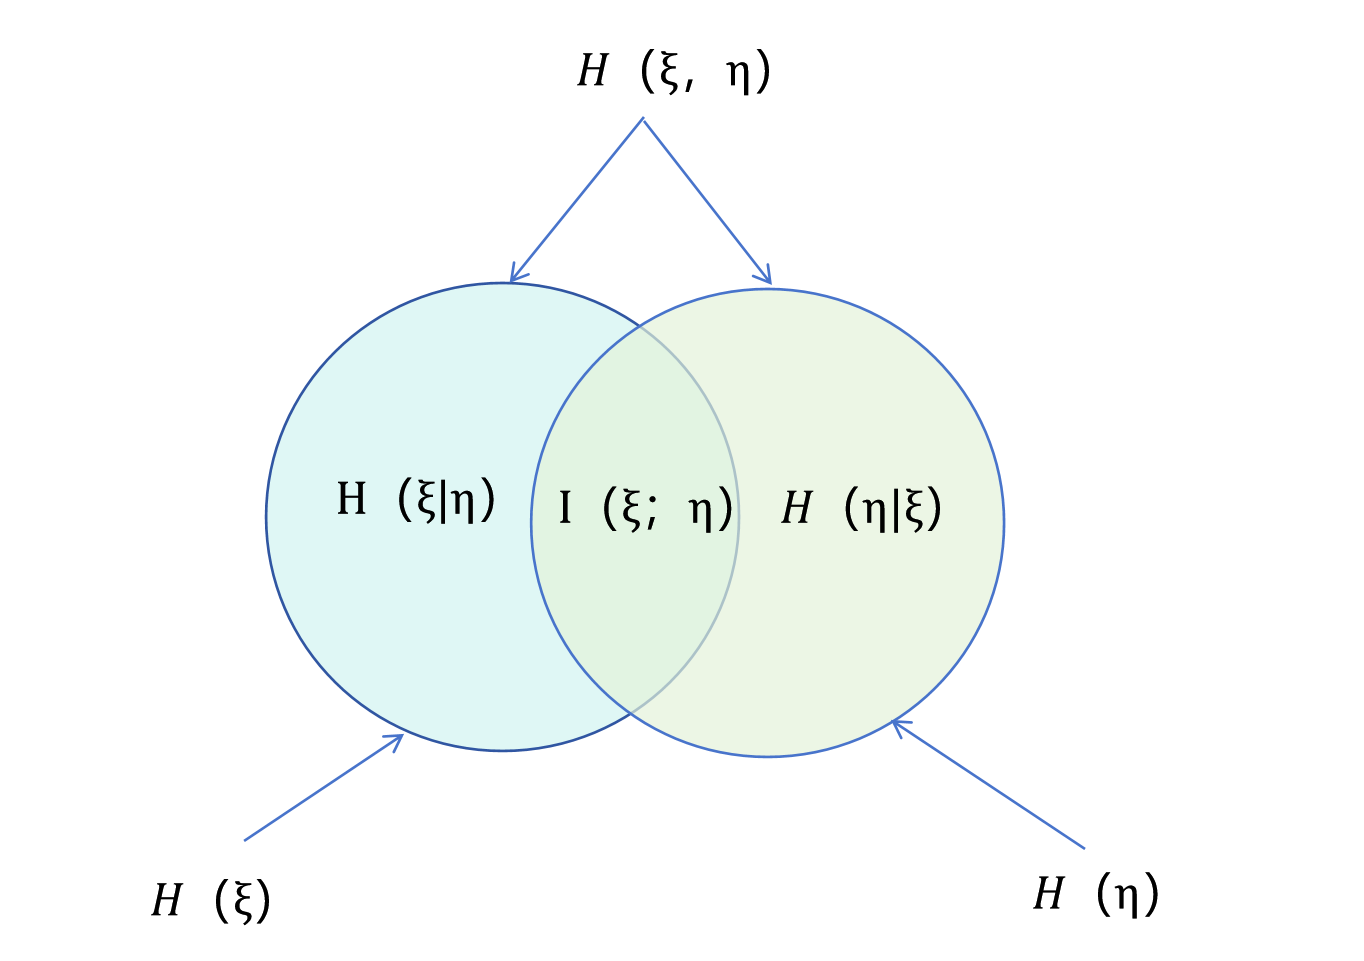
\includegraphics[width=0.4\linewidth]{1.png}
\end{tcolorbox}


\begin{tcolorbox}[breakable,colback=blue!5!white,colframe=blue!75!black,
 title= 2024-03-11]
 设 $ \xi $ 是取 $ m $ 个值 $ x_{1}, x_{2}, \cdots, x_{m} $ 的随机变量, $ p\left(\xi=x_{m}\right)=a $. 证明:
$$
H(\xi)=a \log \frac{1}{a}+(1-a) \log \frac{1}{1-a}+(1-a) H(\eta),
$$
其中 $ \eta $ 是取 $ m-1 $ 个值 $ x_{1},, x_{2}, \cdots, x_{m-1} $ 的随机变量.
$$
p\left(\eta=x_{j}\right) \xlongequal{\text { def }}\frac{p\left(\xi=x_{j}\right)} {(1-a)}, 1 \leqslant j \leqslant m-1 .
$$
进一步, 证
明: $ H(\xi) \leqslant a \log \frac{1}{a}+(1-a) \log \frac{1}{a}+(1-a) \log (m-1) $,并确定其中等号成立的条件.

\tcblower

     证明: 由 $ p\left(\eta=x_{j}\right) \xlongequal{\text { def }}\dfrac{p\left(\xi=x_{j}\right)}{(1-a)}  \Rightarrow p\left(\xi=x_{j}\right)=(1-a) p\left(\eta=x_{j}\right), j=1, \cdots, m-1 . $
$$
\begin{aligned}
\text { 故 } H(\xi)&=a \log \frac{1}{a}+\sum_{j=1}^{m-1} p\left(\xi=x_{j}\right) \log \frac{1}{p\left(\xi=x_{j}\right)} \\
&=a \log \frac{1}{a}+\sum_{j=1}^{m-1}(1-a) p\left(\eta=x_{j}\right) \log \frac{1}{(1-a) p\left(\eta=x_{j}\right)}\\
&=a \log \frac{1}{a}+\sum_{j=1}^{m-1}(1-a) p\left(\eta=x_{j}\right) \log \frac{1}{1-a} +\sum_{j=1}^{m-1}(1-a) p\left(\eta=x_{j}\right) \log \frac{1}{p\left(\eta=x_{j}\right)} \\
&=a \log \frac{1}{a}+(1-a) \log \frac{1}{1-a} \sum_{j=1}^{m-1} p\left(\eta=x_{j}\right) +(1-a) \sum_{j=1}^{m-1} p\left(\eta=x_{j}\right) \log \frac{1}{p\left(\eta=x_{j}\right)} \\
&=a \log \frac{1}{a}+(1-a) \log \frac{1}{1-a}+(1-a) H(\eta)
\end{aligned}
$$

根据熵的最大值定理有 $ H(\eta)\leqslant \log (m-1) $. 因此有
$$ H(\xi) \leqslant a \log \frac{1}{a}+(1-a) \log \frac{1}{a}+(1-a) \log (m-1) $$
等号成立的条件是$ p\left(\eta=x_{j}\right) $ 为等概率分布,
即有
$$
p\left(\eta=x_{j}\right)=\frac{1}{m-1} 
$$
此时$$
 p\left(\xi=x_{j}\right)=\frac{1-a}{m-1}, \quad j=1,2, \cdots, m-1 .
$$

\end{tcolorbox}



\section{第四次课后作业}

\begin{tcolorbox}[breakable,colback=blue!5!white,colframe=blue!75!black,
 title= 单选题]
 码 $ C $ 是前缀码是码 $ C $ 是即时码的( ).

A. 充分条件

B. 充分必要条件

C. 必要条件

\tcblower
(B)

$ \Leftarrow $ : 假设 $ C $ 是一个码元集, 若 $ \mathrm{C} $ 不是前缀码, 则存在码字 $ c_{i}, C_{j} $,使得 $ c_{i} $ 是 $ c_{j} $ 的前缀, 在一个含有 $ c_{i} $ 的码字串中, 从左到右, 当 $ c_{i} $ 出现时,只有当 $ c_{i} $ 后面出现部分, 连同 $ c_{i} $ 不是 $ c_{j} $ 时才能把 $ c_{i} $ 还原;若 $ c_{i} $以及连同后面部分是 $ c_{j} $ 时, 不能把 $ c_{i} $ 还原, 应该把 $ c_{j} $ 还原, 因此 $ C $ 不是即时码,矛盾.故即时码一定为前缀码.
 
$ \Rightarrow $ : 若 $ C $ 不是即时码, 则从左到右, 出现一个码字 $ c_{i} $, 还原为消息字母时, 依赖于后面的字符串, 即存在另一个码字 $ c_{j} $, 使得 $ c_{i} $ 是 $ c_{j} $ 的前缀, 从而C不是前缀码.

\end{tcolorbox}


\begin{tcolorbox}[breakable,colback=blue!5!white,colframe=blue!75!black,
 title= 单选题]
码字长度为 $ \left\{\ell_{1}, \ell_{2}, \cdots, \ell_{a}\right\} $ 的码为即时码是 $ \left\{\ell_{1}, \ell_{2}, \cdots, \ell_{a}\right\} $ 满足Kraft不等式的( ).

A. 充分条件

B. 充分必要条件

C. 必要条件

\tcblower

 若 $ \ell_{1}, \ell_{2}, \cdots, \ell_{2} $ 满足 Kraft不等式, 则必存在码字长度为 $ \ell_{1}, \ell_{2}, \cdots, \ell_{a} $ 的即时码. 如果一个码的码字长度满足 Kraft 不等式, 但它不一定是即时码.

如: 考虑二元码 $ C=\{0,11,100,110\} $,码字长度分别为 $ 1,2,3,3 $,因为$|\mathscr{U}|=2$, 我们有
$$
\frac{1}{2}+\frac{1}{2^{2}}+\frac{1}{2^{3}}+\frac{1}{2^{3}}=1,
$$
所以, 它的码字长度满足kraft 不等式.
但这个码并不是即时的(不是前缀码), 因为码字11是码字110的前缀.
但根据 $ 1,2,3 $, 3 可构造一个即时码,如 $ \{0,10,110,111\} $或 $ \{1,01,001,000\} $.

因此码字长度为 $ \left\{\ell_{1}, \ell_{2}, \cdots, \ell_{a}\right\} $ 的码为即时码是 $ \left\{\ell_{1}, \ell_{2}, \cdots, \ell_{a}\right\} $ 满足Kraft不等式的充分条件.(A)

\end{tcolorbox}



\begin{tcolorbox}[breakable,colback=blue!5!white,colframe=blue!75!black,
 title= 解答题]
 
下面的码是否是即时码? 是否是唯一可译码?\\
(1) $ C=\{0,10,1100,1101,1110,1111\} $.\\
(2) $ C=\{0,10,110,1110,1011,1101\} $.

\tcblower

(1) 在这个码集中,没有任何码字是另一个码字的前缀.因此,每个码字的开始都唯一标识了一个码字,没有歧义,因此是即时码.由于是即时码,它自然也是唯一可译码.即时码的属性保证了解码过程中的唯一性. 故 C 是前缀码, 是即时码, 是唯一可译码.
 
(2) C不是前缀码, 因为码字10是码字1011的前缀, 故C不是即时码.C不是唯一可译码.因为根据如下
字符串得知:一个给定的编码序列中可能会解码出两种不同的消息,表明在这个特定的码集不是唯一可译码.
$$
\frac{0}{a} \frac{10}{b} \frac{110}{c} \frac{1110}{d} \frac{1011}{e} \frac{1101}{\mathrm{f}} $$
$$
\frac{0}{a} \frac{1011}{e} \frac{0}{a} \frac{1110}{d} \frac{1011}{e} \frac{1101}{\mathrm{f}}
$$

\end{tcolorbox}


\begin{tcolorbox}[breakable,colback=blue!5!white,colframe=blue!75!black,
 title= 解答题]
 
判断是否存在即时码具有以下的基数和码字长度, 如果有, 试构造出一个这样的码.\\
(1) $ r=2 $, 长度: 1,3,3,3,4,4.\\
(2) $ r=3 $ ,长度: 1,1,2,2,3,3,3.\\
(3) $ r=5 $, 长度: $ 1,1,1,1,1,8,9 $.


\tcblower

(1) $ r=2 $, 长度: $ 1,3,3,3,4,4 $.

首先,我们计算Kraft和:
$$
\sum_{i=1}^{6} 2^{-\ell_{i}}=2^{-1}+3 \times 2^{-3}+2 \times 2^{-4}=1
$$
Kraft和等于1,满足Kraft不等式,因此存在即时码. 下面构造一个即时码:\\
长度1的码字:0\\
 长度3的码字: $ 100,101,110 $\\
 长度4的码字: 1110,1111

 $$
\begin{array}{lllll}
u_{1,1}=0 & 0 & & &\\
u_{3,1,1}=1 & u_{3,1,2}=0 & u_{3,1,3}=0 & (1,0,0) &\\
u_{3,2,1}=1 & u_{3,2,2}=0 & u_{3,2,3}=1 & (1,0,1) &\\
u_{3,3,1}=1 & u_{3,3,2}=1 & u_{3,3,3}=0 & (1,1,0) &\\
u_{4,1,1}=1 & u_{4,1,2}=1 & u_{4,1,3}=1 & u_{4,1,4}=0 & (1,1,1,0)\\
u_{4,2,1}=1 & u_{4,2,2}=1 & u_{4,2,3}=1 & u_{4,2,4}=1& (1,1,1,1)
\end{array}
$$
故此即时码为
$$
\{0,100,101,110,1110,1111)\}
$$

(2) $ r=3 $, 长度: 1, 1, 2, 2, 3, 3, 3 .

接下来,我们计算Kraft和:
$$
\sum_{i=1}^{7} 3^{-\ell_{i}}=2 \times 3^{-1}+2 \times 3^{-2}+3 \times 3^{-3}=\frac{2}{3}+\frac{2}{9}+\frac{3}{27}=\frac{2}{3}+\frac{2}{9}+\frac{1}{9}=1
$$
Kraft和等于1,满足Kraft不等式,因此存在即时码。下面构造一个即时码:\\
长度1的码字:0,1\\
长度2的码字: 20,21\\
长度3的码字: $ 220,221,222 $

$$
\begin{array}{llrl}
u_{1,1}=0 & u_{1,2}=1 & 0,1&\\
u_{2,1,1}=2 & u_{2,1,2}=0 & (2,0) & \\
u_{2,2,1}=2 & u_{2,2,2}=1 & (2,1) & \\
u_{3,1,1}=2 & u_{3,1,2}=2 & u_{3,1,3}=0 & (2,2,0) \\
u_{3,2,1}=2 & u_{3,2,2}=2 & u_{3,2,3}=1 & (2,2,1) \\
u_{3,3,1}=2 & u_{3,3,2}=2 & u_{3,3,3}=2 & (2,2,2)
\end{array}
$$

故此即时码为
$$
\{0,1,20,21,220,221,222\}
$$

(3)我们计算Kraft和:
$$
\sum_{i=1}^{7} 5^{-\ell_{i}} =5 \times \frac{1}{5}+\frac{1}{5^{8}}+\frac{1}{5^{9}}>1
$$
故这样的即时码不存在.


\end{tcolorbox}




\section{第五次课后作业}

\begin{tcolorbox}[breakable,colback=blue!5!white,colframe=blue!75!black,
 title= 解答题]
 对下面给定的概率分布和基数, 找出一个Huffman编码, 并求平均码长.
$$
p=\{0.1,0.1, \cdots, 0.1\}, r=3 .
$$

\tcblower
解: 首先确定 $ {k} $ 的值,$a=10,r=3$.
$$
k=\operatorname{I n t}_{+}\left(\frac{a-1}{r-1}\right)=\operatorname{I n t}_{+}\frac{9}{2}=5.
$$
再确定第一列最后几个分量相加:$a-(k-1) r+k-1 =10-(5-1) \times 3+5-1=2 $.从第三列开始每次将最后 $r$ 个分量相加,并按大小排序放入下一奇数列.于是我们构造Huffman编码为

\begin{center}
\begin{tabular}{ll||ll||ll||ll||ll} 
\hline
概率 & 码 & 概率 & 码 & 概率 & 码 &概率 & 码 &概率 & 码 \\
\hline
0.1 & 01 & $\boxed{0.2}$ & 00 & $\boxed{0.3}$ & 2 &$\boxed{0.3}$ & 1 &\boxed{0.4} &0  \\
0.1 & 02 & 0.1 & 01 &  0.2  & 00 &0.3 & 2 &0.3 &1 \\
0.1 & 10 & 0.1 & 02 & 0.1 & 01 &0.2 & 00 &0.3 &2 \\
0.1 & 11 & 0.1 & 10 & 0.1 & 02 &0.1 &01  & & \\
0.1 & 12 & 0.1 & 11 & 0.1 & 10 &0.1 &02  & & \\
0.1 & 20 & 0.1 & 12 & 0.1 & 12 & &  & &  \\
0.1 & 21 & 0.1 & 20 & 0.1 &  &  & &\\
0.1 & 22 & 0.1 & 21 &  &  & & & &\\
0.1 & 000 & 0.1 & 22 &  &  & & & &\\
0.1 & 001 &  &  & & & & & &\\
\hline
\end{tabular}
\end{center}

平均码长:
$$L(\mathscr{S}, f)=0.8 \times 2+0.2 \times 3=2.2 $$


\end{tcolorbox}


\begin{tcolorbox}[breakable,colback=blue!5!white,colframe=blue!75!black,
 title= 解答题]
 对下面给定的概率分布和基数,找出一个Huffman编码, 并求平均码长.
$$
\begin{array}{l}
p=\{0.3,0.1,0.1,0.1,0.1,0.06,0.05,0.05,0.05,0.04,0.03,0.02\}, 
\quad r=4 .
\end{array}
$$

\tcblower
解: 首先确定 $ {k} $ 的值,$a=12,r=4$.
$$
k=\operatorname{I n t}_{+}\left(\frac{a-1}{r-1}\right)=\operatorname{I n t}_{+}\frac{11}{3}=4.
$$
再确定第一列最后几个分量相加:$a-(k-1) r+k-1 =12-(4-1) \times 4+4-1=3 $.从第三列开始每次将最后 $r=4$ 个分量相加,并按大小排序放入下一奇数列,用方框标出.于是我们构造Huffman编码为

\begin{center}
\begin{tabular}{ll||ll||ll||ll} 
\hline
概率 & 码 & 概率 & 码 & 概率 & 码& 概率 & 码 \\
\hline
0.3 & 1 & 0.3 & 1 & 0.3 & 1&$\boxed{0.39}$ &0 \\
0.1 & 3 & 0.1 & 3 & $\boxed{0.21}$ & 2 &0.3 &1 \\
0.1 & 00 & 0.1 & 00 & 0.1 & 3 &0.21 &2 \\
0.1 & 01 & 0.1 & 01 &0.1 &00 &0.1 &3 \\
0.1 & 02 & 0.1 & 02 &0.1 &01 & & \\
0.06 & 20 &$\boxed{0.09}$ &03 &0.1 &02 & & \\
0.05 & 21 &0.06 &20 &0.09 &03 & & \\
0.05 & 22 &0.05 &21 & & & & \\
0.05 & 23 &0.05 &22 & & & & \\
0.04 & 030 &0.05 &23 & & & & \\
0.03 & 031 & & & & & & \\
0.02 & 032 & & & & & & \\
\hline
\end{tabular}
\end{center}
平均码长:
$$ L(\mathscr{S}, f)=0.4\times 1+0.51 \times 2+0.09 \times 3=1.69 $$
\end{tcolorbox}


\newpage
\begin{tcolorbox}[breakable,colback=blue!5!white,colframe=blue!75!black,
 title= 解答题]
 判断是否存在即时码具有以下的基数和码字长度, 如果有,试构造出一个这样的码.
$ r=3 $, 长度 $ 1,1,2,4,4,5 $.

\tcblower
我们计算Kraft和:
$$
\sum_{i=1}^{6} 3^{-\ell_{i}}=2 \times 3^{-1}+1 \times 3^{-2}+2 \times 3^{-4}+1 \times 3^{-5}=\frac{2}{3}+\frac{1}{9}+\frac{2}{81}+\frac{1}{243}=\frac{196}{243}<1
$$
满足Kraft不等式,因此存在即时码. 下面构造一个即时码:
$$
\begin{array}{llllll}
u_{1,1}=0 & u_{1,2}=1 & &&&0,1\\
u_{2,1,1}=2 & u_{2,1,2}=0 &&&& (2,0)  \\
u_{4,1,1}=2 & u_{4,1,2}=1 & u_{4,1,3}=0&u_{4,1,4}=0&&(2,1,0,0)  \\
u_{4,2,1}=2 & u_{4,2,2}=1 & u_{4,2,3}=0&u_{4,2,4}=1&&(2,1,0,1)  \\
u_{5,1,1}=2 & u_{5,1,2}=1 & u_{5,1,3}=1 & u_{5,1,4}=0& u_{5,1,5}=0& (2,1,1,0,0) \\
\end{array}
$$
故此即时码为
$$
\{0,1,20,21,2100,2101,21100\}
$$
\end{tcolorbox}


\begin{tcolorbox}[breakable,colback=blue!5!white,colframe=blue!75!black,
 title= 解答题]
对下面给定的概率分布和基数,找出一个Huffman编码,并求平均码长.
$$
p=\{0.3,0.2,0.2,0.1,0.1,0.1\}, \quad r=2 .
$$

\tcblower
解: 首先确定 $ {k} $ 的值,$a=6,r=2$.
$$
k=\operatorname{I n t}_{+}\left(\frac{a-1}{r-1}\right)=\operatorname{I n t}_{+}\frac{5}{1}=5.
$$
再确定第一列最后几个分量相加:$a-(k-1) r+k-1 =6-(5-1) \times 2+5-1=2 $.从第三列开始每次将最后 $r=2$ 个分量相加,并按大小排序放入下一奇数列,用方框标出.于是我们构造Huffman编码为

\begin{center}
    \begin{tabular}{ll||ll||ll||ll||ll}
\hline 概率 & 码 & 概率 & 码 & 概率 & 码 & 概率 & 码& 概率 & 码\\
\hline 0.3 & 01 & 0.3 &01 & $\boxed{0.3}$ & 00 &$\boxed{0.4}$ &1 &$\boxed{0.6}$ &0\\
0.2 & 11 & $\boxed{0.2}$ & 10 & 0.3 & 01 &0.3 &00 &0.4 &1  \\
0.2 & 000 & 0.2 & 11 & 0.2 & 10 &0.3 &01 & &  \\
0.1 & 001 & 0.2 & 000 &0.2 &11 & & & &  \\
0.1 & 100 & 0.1 & 001 & & & & & &  \\
0.1 & 101 & & & & & & & &  \\
\hline
\end{tabular}
\end{center}
平均码长:
$$ L(\mathscr{S}, f)=0.5\times 2+0.5 \times 3=2.5 $$
\end{tcolorbox}

 
\begin{tcolorbox}[breakable,colback=blue!5!white,colframe=blue!75!black,
 title= 判断题]

无噪声信道的容量是 $ \log a $,其中 $ a $ 是输入字母表的大小.
\tcblower
对. 无噪声信道等价条件是, 存在一个 $ \mathscr{U} \rightarrow \mathscr{V} $ 的 $ 1-1 $ 映射 $ \phi $, 使得 $ p(\phi(u) \mid u)=1 $ 对所有 $ u $ 成立, 从而 $ a=b $. 因此 $ C=\log a=\log b $.
\end{tcolorbox}



\begin{tcolorbox}[breakable,colback=blue!5!white,colframe=blue!75!black,
 title= 判断题]

无用信道的容量是 0 .
\tcblower
对.  无用信道意味着输出不依赖于输入,或者说输出对于输入的选择完全没有信息.在这种情况下,无论输入是什么,输出的分布都保持不变,因此 \(H(\eta | \xi) = H(\eta)\). $ I(\xi ; \eta)=H(\xi)-H(\xi \mid \eta)=H(\xi)-H(\xi)=0 $. (注意 $ \xi $ 与 $ \eta $ 是相互独立的.)
\end{tcolorbox}

\begin{tcolorbox}[breakable,colback=blue!5!white,colframe=blue!75!black,
 title= 判断题]

无丢失信道的容量是 $ \log a $, 其中 $ a $ 是输入字母表的大小.
\tcblower
对.  因  $\xi$  完全由  $\eta$决定,即 $ H(\xi \mid \eta)=0 $.
$$
\begin{aligned}
I(\xi ; \eta)  =H(\xi)-H(\xi \mid \eta)  =H(\xi)-0  =H(\xi) \leq \log a
\end{aligned}
$$
$ H(\xi) $ 的最大值 $ \log a $.
\end{tcolorbox}

\begin{tcolorbox}[breakable,colback=blue!5!white,colframe=blue!75!black,
 title= 解答题]

写出二元对称信道的信道矩阵, 并利用信道容量的定义求它的信道容量.
\tcblower

记输入输出字母表 $ \mathscr{U}=\mathscr{V}=\{0,1\} $. 信道转移概率分布为
$$
p(0 \mid 1)=p(1 \mid 0)=p, p(0 \mid 0)=p(1 \mid 1)=1-p
$$
则二元对称信道的信道矩阵如下所示:
$$
\begin{array}{ccc}
 & 0 & 1 \\
0 & 1-p & p \\
1 & p & 1-p
\end{array}
$$
下面利用信道容量的定义求它的信道容量. 
$$C=\max \left\{I(\xi ; \eta) \mid \xi \in \mathscr{P}_{\mathscr{U}}\right\}=\max \left\{H(\eta)-H(\eta \mid \xi) \mid \xi \in \mathscr{P}_{\mathscr{U}}\right\}$$

设入口分布为 $\left(p_{0}, p_{1}\right)$, 对应的出口分布为 $\left(q_{0}, q_{1}\right)$,则
$$
\begin{aligned}
\left(q_{0}, q_{1}\right) & =\left(p_{0}, p_{1}\right)\left(\begin{array}{cc}
1-p & p \\
p & 1-p
\end{array}\right) =\left(p_{0}(1-p)+p_{1}  p,\quad p_{0} p+p_{1}(1-p)\right)
\end{aligned}
$$
不妨设 $p_{0}=\theta ,$ 则 $ p_{1}=1-\theta, 0 \leqslant \theta \leqslant 1 $.
$$ \begin{aligned} q_{0} & =\theta(1-p)+(1-\theta) p=\theta+p-2 \theta p \\ q_{1} & =\theta p+(1-\theta)(1-p)=1-\theta-p+2 \theta p \\ H(\eta) & =-q_{0} \log _{2} q_{0}-q_{1} \log _{2} q_{1} \\ & =-q_{0} \log _{2} q_{0}-\left(1-q_{0}\right) \log _{2}\left(1-q_{0}\right) \\ & =H\left(q_{0}\right)\end{aligned} $$

 根据熵函数的性质$q_{0}$ 取$\frac 12$ 时 $H(\eta) $最大且取值为 $1$, 此时 $q_0= \theta+p-2 \theta p=\frac{1}{2} $, 化简即得 $ \theta=\frac{1}{2} $.

由于
$$
\begin{aligned}
H(\eta \mid \xi=0) & =p(0 \mid 0) \log \frac{1}{p(0 \mid 0)}+p(1 \mid 0) \log \frac{1}{p(1 \mid 0)} \\
& =(1-p) \log \frac{1}{1-p}+p \log \frac{1}{p}=H(p) \\
H(\eta \mid \xi=1) & =p(0 \mid 1) \log \frac{1}{p(0 \mid 1)}+p(1 \mid 1) \log \frac{1}{p(1 \mid 1)} \\
& =p \log \frac{1}{p}+(1-p) \log \frac{1}{1-p}=H(p) .
\end{aligned}
$$
所以
$$H(\eta \mid \xi)=\sum_{u \in \mathscr{U}} p(u) H(\eta \mid \xi=u)=\sum_{u \in \mathscr{U}} p(u) H(p)=\left(\sum_{u \in \mathscr{U}} p(u)\right) H(p)=H(p)$$

因此二元对称信道的信道容量为
$$C=\max \left\{H(\eta)-H(\eta \mid \xi) \right\}=1-H(p)$$

\end{tcolorbox}



\begin{tcolorbox}[breakable,colback=blue!5!white,colframe=blue!75!black,
 title= 解答题]

考虑离散无记忆信道 $ Y=(X+Z) \bmod 11 $, 其中
$$
Z=\left(\begin{array}{ccc}
1 & 2 & 3 \\
\frac1 3 & \frac1 3 &\frac1 3
\end{array}\right)
$$
$ X \in\{0,1, \cdots, 10\} $. 假设 $ X $ 和 $ Z $ 独立.\\
(1) 求这个信道的容量.\\
(2) 找出达到信道容量的入口分布.
\tcblower

(1) $ Y=(X+Z) \bmod 11 $, 输入为 $ X $, 输出为 $ Y, Z $ 为噪声信道, 而
$
Z=\left(\begin{array}{ccc}
1 & 2 & 3 \\
\frac1 3 & \frac1 3 & \frac1  3
\end{array}\right), \quad X \in\{0,1, \cdots, 10\}.
$
所以 $ Y \in\{0,1, \cdots, 10\} $, 

因为 $ Z $ 可以取三个值 $ (1,2,3) $ ,每个都有 $ \frac{1}{3} $ 的概率,所以对于每个 $ X $ 的值, $ Y $ 可以是三个可能的结果之一,这取决于 $ Z $ 的值.信道矩阵 $ P(Y \mid X) $ 将具有 11 行 (对应于 $ X $ 的可能值) 和 11 列(对应于 $ Y $ 的可能值).每个元素 $ P_{i j} $ 表示给定输入 $ X=i $ 时输出 $ Y=j $ 的概率.

由于 $ Z $ 的作用是加在 $ X $ 上然后对 11 取模,每个 $ X $ 值将映射到三个不同的 $ Y $ 值,每个的概率都是 $ \frac{1}{3} $ .例如,如果 $ X=0 $ ,则 $ Y $ 可以是 $ 1 , 2 $ 或 3 ,每个都有 $ \frac{1}{3} $ 的概率,因为 $ Z $ 分别加 $ 1 , 2 $ 或 3 .因此,信道矩阵的一般形式将是每行有三个 $ \frac{1}{3} $ 的条目,分别对应于 $ X $ 加上 $ 1 , 2 , 3 $ 和模 11 的结果,而其他位置为 0 .对于 $ X=0: Y $ 的可能值是 $ 1,2,3 $ ,每个概率为 $ \frac{1}{3} $ . 对于 $ X=1: Y $ 的可能值是 $ 2,3,4 $ ,每个概率为 $ \frac{1}{3} $ .以此类推,直到 $ X=10 $ .每行的具体值会随着 $ X $ 的增加而“滚动”,并在达到 10 并绕回 0 时循环.这种模式的重复构成了完整的信道矩阵:

\begin{center}
     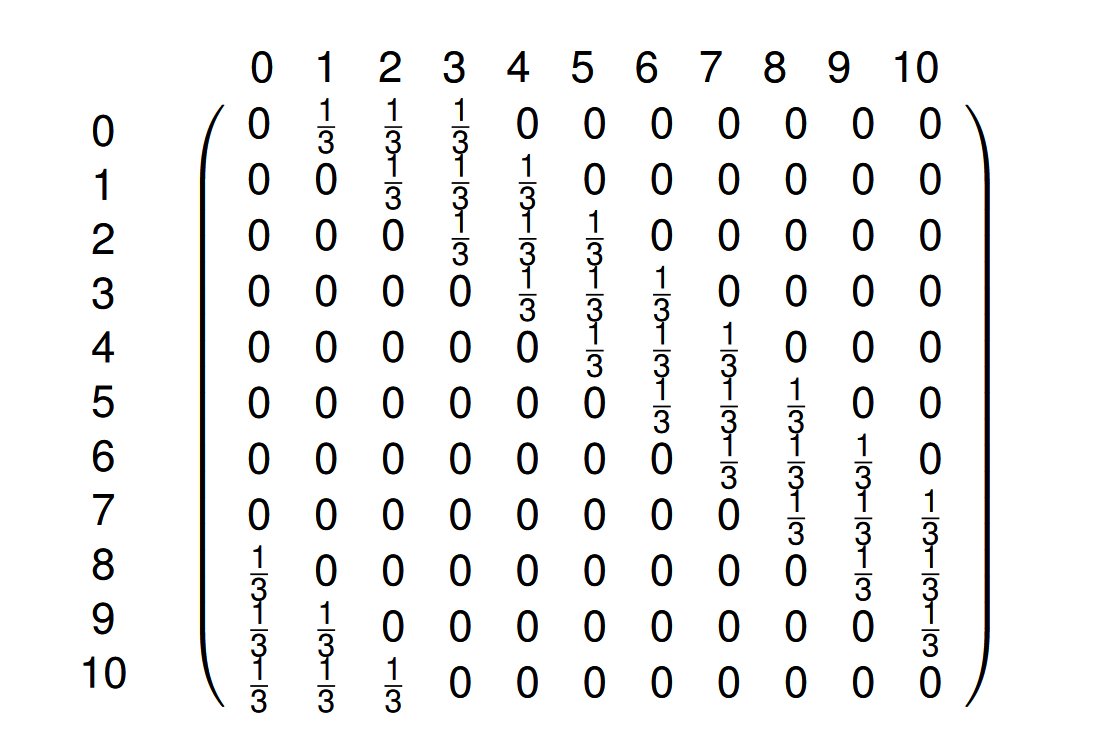
\includegraphics[width=0.4\linewidth]{2.png}
\end{center}

得到一个对称信道,在这种情况下,
$$
H(Y \mid X)=H(Z \mid X)=H(Z)=\left(\frac{1}{3} \log 3+\frac{1}{3} \log 3+\frac{1}{3} \log 3\right) =\log 3,
$$
与$ X $的分布无关,因此信道的容量为
$$
\begin{aligned}
C  =\max _{p(x)} I(X ; Y) & =\max _{p(x)} H(Y)-H(Y \mid X) \\
& =\max _{p(x)} H(Y)-\log 3 \\
& =\log 11-\log 3= \log \frac{11}{3}
\end{aligned}
$$

(2) 当$ Y $具有均匀分布时达到最大值,根据对称性知道, 这发生在$ X $具有均匀分布时,即
$$
p(X)=\frac{1}{11}, \quad, X \in\{0,1, \cdots, 10\} .
$$



\end{tcolorbox}




\begin{tcolorbox}[breakable,colback=blue!5!white,colframe=blue!75!black,
 title= 解答题]

写出二元对称信道, 二元擦除信道及 $ M $ 信道的信道矩阵.
\tcblower

    \centering
    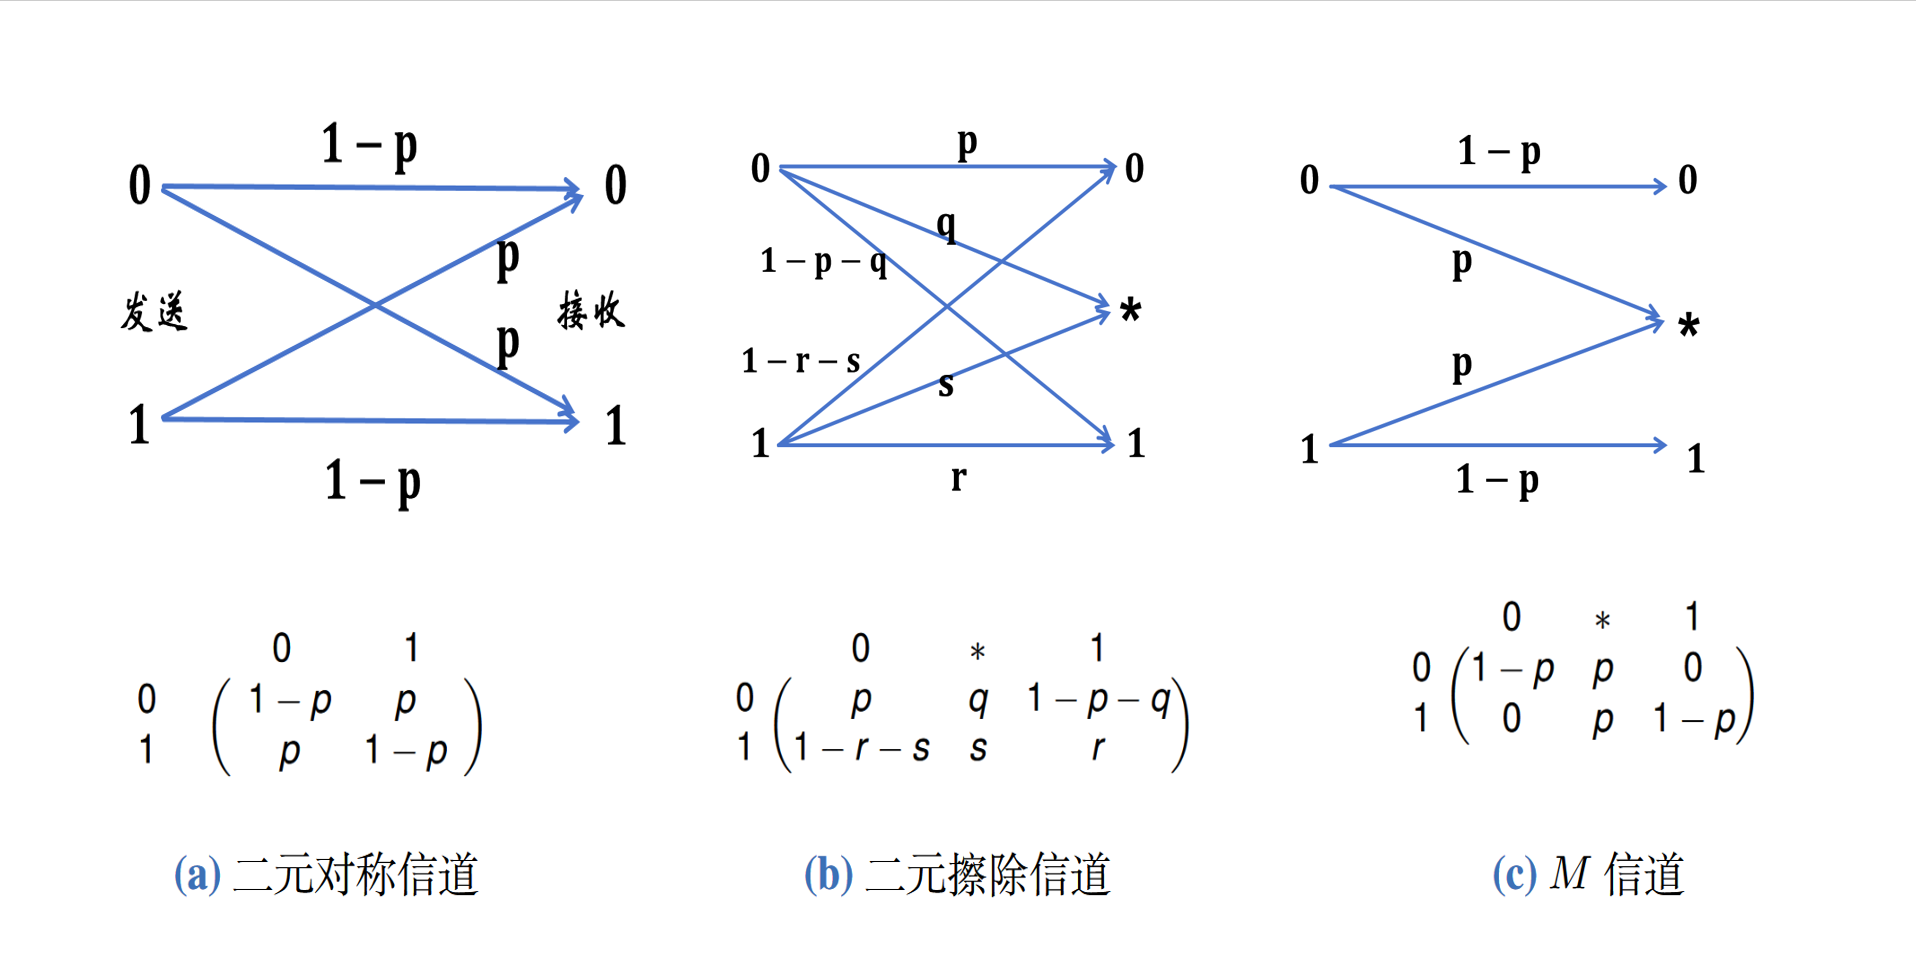
\includegraphics[width=1\linewidth]{3.png}
    
\end{tcolorbox}




\begin{tcolorbox}[breakable,colback=blue!5!white,colframe=blue!75!black,
 title= 解答题]

写出二元对称信道的信道矩阵, 并利用极值法求它的信道容量.
\tcblower

   二元对称信道的信道矩阵为 $ \left(\begin{array}{cc}1-p & p\\ p & 1-p\end{array}\right) $. 设入口分布为 $ \left(p_{0}, p_{1}\right) $,对应的出口分布为 $ \left(q_{0}, q_{1}\right) $ ,则 $ \left(q_{0}, q_{1}\right)=\left(p_{0}, p_{1}\right)\left(\begin{array}{cc}1-p & p \\ p & 1-p\end{array}\right)=\left(p_{0}(1-p)+p_{1} \cdot p, p_{0} p+(1-p) p_{1}\right) $
$$
\begin{aligned}
C & =\sum_{j=1}^{b} p\left(v_{j} \mid y_{i}\right) \log \frac{p\left(v_{j} \mid u_{i}\right)}{q\left(v_{j}\right)} \\
& =(1-p) \log \frac{1-p}{q_{0}}+p \log \frac{p}{q_{1}} \\
& =p \log \frac{p}{q_{0}}+(1-p) \log \frac{1-p}{q_{1}}
\end{aligned}
$$

展开有 $ \log \frac{1-p}{q_{0}}-p \log \frac{1-p}{q_{0}}+p \log \frac{p}{q_{1}}=p \log \frac{p}{q_{0}}+\log \frac{1-p}{q_{1}}-p \log \frac{1-p}{q_{1}} $
$$
\begin{aligned}
\log \frac{q_{1}}{q_{0}}+p \log \frac{q_{0}}{q_{1}}+p \log \frac{q_{0}}{q_{1}} & =0 \\
(2 p-1) \log \frac{q_{0}}{q_{1}} & =0
\end{aligned}
$$
则 $ p=\frac{1}{2} $ 或 $ q_{0}=q_{1} $.
由 $ q_{0}=q_{1} $ 知 $p_{0}(1-p)+p_{1}-p=p_{0} p+(1-p) p_{1}$ $\Rightarrow p=\frac{1}{2} \text { 或 } p_{1}=p_{0}$.
由 $ p_{0}+p_{1}=1 $ 知 $ p_{0}=p_{1}=\frac{1}{2} $ 进而 $ q_{0}=q_{1}=\frac{1}{2} $
于是
$$
\begin{aligned}
C & =p \log \frac{p}{\frac{1}{2}}+(1-p) \log \frac{1-p}{\frac{1}{2}} \\
& =p \log 2 p+(1-p) \log 2(1-p) \\
& =p+p \log p+1-p+(1-p) \log (1-p) \\
& =1+p \log p+(1-p) \log (1-p) \\
& =1-H(p)
\end{aligned}
$$
    
\end{tcolorbox}


\newpage
\begin{tcolorbox}[breakable,colback=blue!5!white,colframe=blue!75!black,
 title= 解答题]

写出 $ M $ 信道的信道矩阵, 并利用极值法求它的信道容量.
\tcblower

   $ M $ 信道的信道矩阵为 $ \left(\begin{array}{ccc}1-p & p & 0 \\ 0 & p & 1-p\end{array}\right) $.
设入口分布为 $ \left(p_{0}, p_{1}\right) $,对应的出口分布为 $ \left(q_{0}, q_{1}, q_{2}\right)$, 且$q\left(v_{j}\right)=\sum\limits_{i=1}^{a} p\left(u_{i}\right) {p}\left(v_{j} \mid u_{i}\right) $
则有
$$
\begin{array}{c}
\left(q_{0}, q_{1}, q_{2}\right)=\left(p_{0}, p_{1}\right)\left(\begin{array}{ccc}
1-p & p & 0 \\
0 & p & 1-p
\end{array}\right)=\left(p_{0}(1-p),\left(p_{0}+p_{1}\right) p, p_{1}(1-p)\right)
\end{array}
$$
$$
\begin{aligned}
C& =\sum_{j=1}^{b} p\left(v_{j} \mid u_{i}\right) \log \frac{p\left(v_{j} \mid u_{i}\right)}{\sum\limits_{l=1}^{a} p\left(u_{i}\right) p\left(y_{j} \mid u_{l}\right)} \\
& =\sum_{j=1}^{b} p\left(v_{j} \mid u_{i}\right) \log \frac{p\left(v_{j} \mid u_{i}\right)}{q\left(v_{j}\right)} \\
& =(1-p) \cdot \log \frac{1-p}{q_{0}}+p\log \frac{p}{p_{i}} \\
& =p \log \frac{p}{q_{1}}+(1-p) \cdot \log \frac{1-p}{q_{2}}
\end{aligned}
$$

根据上面等式,比对后有 $ (1-p) \log \frac{1-p}{q_{0}}=(1-p) \cdot \log \frac{1-p}{q_{2}} $.
即得 $ q_{0}=q_{2} $.

于是 $ p_{0}(1-p)=p_{1}(1-p) \Rightarrow p_{0}=p_{1} $
由 $ p_{0}+p_{1}=1 $ 知 $ p_{0}=p_{1}=\frac{1}{2}$,则$q_{0}=p_{0}(1-p)=\frac{1-p}{2} $.
同理 $ q_{1}=p, q_{2}=\frac{1-p}{2} $, 将 $ q_{0}, q_{1}, q_{2} $ 的值代回等式中,于是 
$$
\begin{aligned}
 C&=p \log \frac{p}{q_{1}}+(1-p) \log \frac{1-p}{q_{2}} \\
&=p \log \frac{p}{p}+(1-p) \log \frac{1-p}{\frac{1-p}{2}} \\
&=(1-p) \log 2=1-p
\end{aligned}
$$
    
\end{tcolorbox}


\newpage
\begin{tcolorbox}[breakable,colback=blue!5!white,colframe=blue!75!black,
 title= 解答题]

$Z$信道如下图所示, 写出它的信道矩阵并求其信道容量.

\begin{center}
    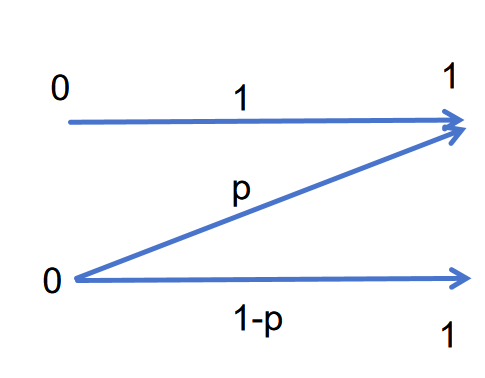
\includegraphics[width=0.2\linewidth]{4.png}
\end{center}


\tcblower

   信道矩阵为 $ \left(\begin{array}{cc}1 & 0 \\ p & 1-p\end{array}\right) $.
设入口分布为 $ \left(p_{0}, p_{1}\right) $ ,对应的出口分布为 $ \left(q_{0}, q_{1}\right) $,则 
$$ \left(q_{0}, q_{1}\right)=\left(p_{0}, p_{1}\right)\left(\begin{array}{cc}1 & 0 \\ p & 1-p\end{array}\right)=\left(p_{0}+p_{1} p, p_{1}(1-p)\right) $$
$$
\begin{aligned}
c & =\sum_{j=1}^{b} p\left(v_{j} \mid v_{i}\right) \log \frac{p\left(v_{j} \mid u_{i}\right)}{q\left(v_{j}\right)} \\
& =1 \cdot \log \frac{1}{q_{0}} \\
& =p \cdot \log \frac{p}{q_{0}}+(1-p) \log \frac{1-p}{q_{1}}
\end{aligned}
$$

根据等式有 $ -\log q_{0}=p \cdot \log \frac{p}{q_{0}}+(1-p) \cdot \log \frac{1-p}{q_{1}} $
$$
\begin{aligned}
-\log q_{0} & =p \log p-p \log q_{0}+(1-p) \log (1-p)-(1-p) \log q_{1} \\
H(p) & =(1-p) \log \frac{q_{0}}{q_{1}}
\end{aligned}
$$

于是 $ \frac{q_{0}}{q_{1}}=e^{\frac{H(p)}{1-p}} $.
由于 $ q_{0}+q_{1}=1 $ ,所以 $ \frac{1-q_{1}}{q_{1}}=e^{\frac{H(p)}{1-p}} $, 令 $ \lambda=\frac{H(p)}{1-p} $
解得 $ q_{1}=\frac{1}{1+e^{\lambda}} $, 则 $ q_{0}=\frac{e^{\lambda}}{1+e^{\lambda}} $
$$
\begin{aligned}
C=\log \frac{1}{q_{0}}=\log \frac{1+e^{\lambda}}{e^{\lambda}} & =\log \left(1+\frac{1}{e^{\lambda}}\right) \\
& =\log \left(1+e^{-\frac{H(p)}{1-p}}\right)
\end{aligned}
$$
    
\end{tcolorbox}
\newpage
\section{第八次课后作业}
\begin{tcolorbox}[breakable,colback=blue!5!white,colframe=blue!75!black,
 title= 选择题]

设 $C$ 是一个 $q$ 元 $ (n, M, d) $ 码,则 $C$ 的码率是$(\quad )$

 $A. \dfrac{M}{n} $ $\qquad$  $B. \dfrac{\log _{{q}}{M}}{{n}} $


 \tcblower
对于一个 $q$ 元 $(n, M, d)$ 码,其中 $n$ 为码字长度,$M$ 为码字个数,$d$ 为最小距离,码率 $R(C)$ 定义为有效信息位与总位数之比,即 $R(C) = \frac{k}{n}$,其中 $k = \log_{q} M$ 为每个码字中的有效信息位数.

因此,码率 $R(C)$ 可表示为 $R(C) = \frac{\log_{q} M}{n}$,选项 $B. \frac{\log_{q} M}{n}$ 是正确的.
 \end{tcolorbox}


\begin{tcolorbox}[breakable,colback=blue!5!white,colframe=blue!75!black,
 title= 选择题]

设二元码 $ C=\{1100,0101,1010\} $ ,则码 $ C $ 的最小距离是 $(\quad )$

$A. 1 \qquad  B. 2 \qquad  C. 3$

 \tcblower
对于二元码 $ C=\{1100,0101,1010\} $,我们需要计算所有可能的码字对之间的Hamming距离,并找出最小的距离.给定码 $ C $,我们可以计算得到: $d(1100, 0101) = 2$, $d(1100, 1010) = 2$, $d(0101, 1010) = 4$. 因此,码 $ C $ 的最小距离为 $ d(C) = 2 $.所以选项 $B. 2$ 是正确的.
 \end{tcolorbox}


\begin{tcolorbox}[breakable,colback=blue!5!white,colframe=blue!75!black,
 title= 选择题]

 设 $ C $ 是一个二元 $ (5,4,3) $ 码,则 $ C $ 至多可纠正的错误个数$(\quad )$

$A. 1 \qquad  B. 2 \qquad  C. 3$

 \tcblower
对于一个二元 $(n, M, d)$ 码,其最大可纠正的错误个数为 $t = \lfloor \frac{d-1}{2} \rfloor$.在这里,$d=3$,所以最大可纠正的错误个数为 $t = \lfloor \frac{3-1}{2} \rfloor = 1$.

因此,$C$ 是一个二元 $(5, 4, 3)$ 码,至多可纠正的错误个数为 $1$,选项 $A. 1$ 是正确的.

(定理:码$C$至多可纠正$t$个错误的充分必要条件为$d(C)=2t+1$或$d(C)=2t+2$.)
 \end{tcolorbox}


 \begin{tcolorbox}[breakable,colback=blue!5!white,colframe=blue!75!black,
 title= 选择题]

设 $ C $ 是一个二元 $ (7 , 16 , 3 )$  码(如三阶二元Hamming码),则 $C$ 至多可检查的错误个数是$(\quad )$

$A. 1 \qquad  B. 2 \qquad  C. 3$
 \tcblower
根据定理:码$C$至多可检查$t$个错误的充分必要条件为$d(C)=t+1$.

因此,对于二元 $(7, 16, 3)$ 码,至多可检查的错误个数为 $2$,选项 $B. 2$ 是正确的.
 \end{tcolorbox}


\newpage
 \begin{tcolorbox}[breakable,colback=blue!5!white,colframe=blue!75!black,
 title= 解答题]

设 $ C=\{11100,01001,10010,00111\} $ 是一个二元 $ (5,4) $ 码

(1) 求码 $ C $ 的最小距离.

(2)根据最小距离译码原则,对接收到的字 10000,01100 , 00100分别进行译码.

(3)计算码 $ C $ 的码率.
 \tcblower
(1)
要求码 $ C $ 的最小距离,我们需要计算所有可能的码字对之间的Hamming距离,并找出最小的距离.给定码 $ C=\{11100,01001,10010,00111\} \subset V(5,4)$, 令 $x_{1}  =11100, x_{2}=01001, x_{3}=10010, x_{4}=00111 $.我们可以计算得到:
$$
\begin{aligned}
d\left(x_{1}, x_{2}\right) & =3, d\left(x_{1}, x_{3}\right)=3, d\left(x_{1}, x_{4}\right)=4 \\
d\left(x_{2}, x_{3}\right) & =4, d\left(x_{2}, x_{4}\right)=3, d\left(x_{3}, x_{4}\right)=3 \\
\end{aligned}
$$
因此$d(c)=\min \left\{d\left(x_{i}, x_{j}\right) \mid x_{i}, x_{j} \in C, x_{i} \neq x_{j}, i, j=1,2,3,4\right\} =3$

(2) 根据最小距离译码原则,我们选择收到的字与码 $ C $ 中距离最近的码字进行译码.
对于接收到的字 10000:设 $ x=10000 $ ,则
$$
d\left(x, x_{1}\right)=2, d\left(x, x_{2}\right)=3, d\left(x, x_{3}\right)=1, d\left(x, x_{4}\right)=4
$$
因此将 $x$ 译为 $x_{3}$ ,即接收到的字 10000 应当译码为 10010

对于接收到的字 01100:设 $ y=01100 $ ,则
$$
d\left(y, x_{1}\right)=1, d\left(y, x_{2}\right)=2, d\left(y, x_{3}\right)=4, d\left(y, x_{4}\right)=3
$$
因此将 $ y $ 译为 $ x_{1} $. 即 $ 01100 \rightarrow 11100 $

对于接收到的字 00100:设 $ z=00100 $ ,则
$ d\left(z, x_{1}\right)=2, d\left(z, x_{2}\right)=3, d\left(z, x_{3}\right)=3, d\left(z, x_{4}\right)=2 $
因此将$z$ 译为 $ x_{1} $ 或 $ x_{4} $ ,即 $ 00100 \rightarrow 11100 $ 或 $ 00100 \rightarrow 00111 $

(3) 对于二元 $(5,4)$ 码 $ C $,其中 $ M = 4 $(共有4个码字),$ n = 5 $(每个码字长度为5位).根据码率公式 $ R(C) = \frac{\log_{2} M}{n} $,我们有:
$$
R(C) = \frac{\log_{2} 4}{5} = \frac{2}{5}
$$
因此,码 $ C $ 的码率为 $ \frac{2}{5} $.
 \end{tcolorbox}

\newpage
  \begin{tcolorbox}[breakable,colback=blue!5!white,colframe=blue!75!black,
 title= 解答题]

设 $ C=\{00000000,00001111,00110011,00111100\} $ 是一个二元 $ (8,4) $ 码.

(1) 计算码 $ C $ 中不同码字的Hamming距离和码 $ C $ 的最小距离.

(2) 在一个二元码中, 如果把某一个码字中的 0 和 1 互换,即将 0 换为 1,1 换为 0 , 则我们将所得的字称为原码字的补. 一个二元码的所有码字的补构成的集合称为原码的补码. 求码 $ C $ 的补码, 并求补码中所有不同码字之间的Hamming距离和补码的最小距离.它们与(1)中的结果有什么关系?

(3) 将(2)中的结果推广到一般的二元码.
 \tcblower

(1)令 $x_{1}=00000000, x_{2}=00001111, x_{3}=00110011, x_{4}=00111100$ 
$$
\begin{array}{l}
d\left(x_{1}, x_{2}\right)=4, d\left(x_{1}, x_{3}\right)=4, d\left(x_{1}, x_{4}\right)=4 \\
d\left(x_{2}, x_{3}\right)=4, d\left(x_{2}, x_{4}\right)=4, d\left(x_{3}, x_{4}\right)=4 \\
\end{array}
$$
因此 $ d(c)=4 $

(2) 设补码 $ \overline{C}=\{11111111 $ , $ 1110000 , 11001100 , 11000011\} $,
$\overline{C}$ 中的码字分别记作 $ y_{1}, y_{2} , y_{3} , y_{4} $ ,则
$$
\begin{array}{l}
d\left(y_{1}, y_{2}\right)=4, d\left(y_{1}, y_{3}\right)=4, d\left(y_{1}, y_{4}\right)=4 \\
d\left(y_{2}, y_{3}\right)=4, d\left(y_{2}, y_{4}\right)=4, d\left(y_{3}, y_{4}\right)=4
\end{array}
$$
因此 $ d\left(\overline{C}\right)=4 $, 对比(1)可知, $C$ 的补码中码字间
的 Hamming 距离与 $ C $ 相对应的码字间 Hamming
距离相同且 $C$ 的补码的最小距离与 $C$ 的最小距离相同.

(3) 对于一般的二元码,任取原码中两个不同码字 $ x = x_1 x_2 \ldots x_n $ 和 $ y = y_1 y_2 \ldots y_n $,其补码分别为 $ \bar{x} = \bar{x_1} \bar{x_2} \ldots \bar{x_n} $ 和 $ \bar{y} = \bar{y_1} \bar{y_2} \ldots \bar{y_n} $.其中 $ x_i,y_i \in \{0, 1\} $, $ \bar{x_i} = 1 - x_i $, $ \bar{y_i} = 1 - y_i $. $i=1,2,\cdots,n$.
原码 $ x $ 和 $ y $ 之间的Hamming距离为 $ d(x, y) = \sum\limits_{i=1}^{n} |x_i - y_i| $,补码 $ \bar{x} $ 和 $ \bar{y} $ 之间的Hamming距离为 $ d(\bar{x}, \bar{y}) = \sum\limits_{i=1}^{n} |\bar{x_i} - \bar{y_i}| = \sum\limits_{i=1}^{n} |(1 - x_i) - (1 - y_i)| = \sum\limits_{i=1}^{n} |y_i - x_i| = d(x, y) $.
因此,原码 $ x $ 和 $ y $ 之间的Hamming距离与其补码 $ \bar{x} $ 和 $ \bar{y} $ 之间的Hamming距离相等.根据 $x,y$ 的任意性进而得知而补码的最小距离与原码的最小距离相同.
 \end{tcolorbox}
\newpage
\section{第八次课后作业}
\begin{tcolorbox}[breakable,colback=blue!5!white,colframe=blue!75!black,
 title= 填空题]

码 $ C $ 至多可纠正 $ t $ 个错误的充分必要条件是码 $ C $ 的最小距离 $ d(C)= $ $\underline{\hspace{2em}}$.

 \tcblower
定理:码$C$至多可纠正$t$个错误的充分必要条件为$d(C)=2t+1$或$d(C)=2t+2$.
 \end{tcolorbox}



 \begin{tcolorbox}[breakable,colback=blue!5!white,colframe=blue!75!black,
 title= 填空题]

对于任意二元 $ (3, M, 2) $ 码, 一定有 $ M \leq $ $\underline{\hspace{2em}}$.

 \tcblower
使用Singleton界定理可以帮助我们确定编码理论中线性码的一个上界.Singleton界定理指出,对于任意的 \(q\)-元 \((n, M, d)\) 码,其码长为 \(n\)、码字数为 \(M\) 以及最小汉明距离为 \(d\),我们有:

\[
M \leq q^{n-d+1}
\]

对于一个二元 \((3, M, 2)\) 码,其中 \(q = 2\)(因为是二元码)、\(n = 3\)(码字长度为3)和 \(d = 2\)(最小汉明距离为2),因此
   \[
   M \leq 2^{3-2+1} = 2^2 = 4
   \]
 \end{tcolorbox}



 \begin{tcolorbox}[breakable,colback=blue!5!white,colframe=blue!75!black,
 title= 填空题]

设二元 $ [4,2] $ 线性码 $ L=\{0000,1100,0011,1111\} $, 则 $ L $ 的最小距离为 $\underline{\hspace{2em}}$.

 \tcblower
为了找出给定的二元线性码 \( L = \{0000, 1100, 0011, 1111\} \) 的最小距离,我们需要计算码集中任意两个不同码字之间的汉明距离,然后找出这些距离中的最小值.

汉明距离是指两个码字在相应位上不同的位数.对于线性码,最小距离也可以通过找出除了零码字以外的码字的最小重量(即非零位的数量)来得到,因为线性码的任意两个码字的差也是该码中的一个码字.

我们用两种方法分别来计算:

1. 码字重量分析:

   \( 0000 \) 的重量为 \( 0 \)(无需考虑,因为我们寻找的是非零码字的最小重量).
   
    \( 1100 \) 的重量为 \( 2 \).
    
    \( 0011 \) 的重量为 \( 2 \).
    
    \( 1111 \) 的重量为 \( 4 \).

2. 码字间的汉明距离:

    从 \( 0000 \) 到 \( 1100 \),距离为 \( 2 \).
    
    从 \( 0000 \) 到 \( 0011 \),距离为 \( 2 \).
    
    从 \( 0000 \) 到 \( 1111 \),距离为 \( 4 \).
    
    从 \( 1100 \) 到 \( 0011 \),距离为 \( 4 \).
    
    从 \( 1100 \) 到 \( 1111 \),距离为 \( 2 \).
    
    从 \( 0011 \) 到 \( 1111 \),距离为 \( 2 \).

由上面的计算可见,码字之间的最小汉明距离是 \( 2 \),这也是该码的最小距离.因此,给定的二元线性码 \( L \) 的最小距离为 \( 2 \).
 \end{tcolorbox}


 \begin{tcolorbox}[breakable,colback=blue!5!white,colframe=blue!75!black,
 title= 填空题]

对于任意 $ n \geq 1, \quad A_{q}(n, n)= $  $\underline{\hspace{2em}}$.

 \tcblower
设 $ C $ 是一个 $ q $ 元 $ (n, M, n) $ 码, 则 $ \forall x, y \in C, x=\left(x_{1}, \cdots, x_{n}\right), y=\left(y_{1}, \cdots, y_{n}\right), x_{i} \neq y_{i}, i=  1, \cdots, n $, 因此, 所有码字在一个固定分量位置上出现的字符一定互不相同, 于是 $ M \leq q $. 由此可知 $ A_{q}(n, n) \leq q $, 又码长为 $ n $ 的 $ q $ 元重复码是一个 $ q $ 元 $ (n, q, n) $ 码, 故 $ A_{q}(n, n)=q $.
 \end{tcolorbox}


 \begin{tcolorbox}[breakable,colback=blue!5!white,colframe=blue!75!black,
 title= 解答题]

(1) 证明: 对任意三元 $ (3, M, 2) $ 码, 一定有 $ M \leq 9 $.

(2) 证明: 三元 $ (3,9,2) $ 码一定存在. 于是, $ A_{3}(3,2)=3^{2} $.

(3) 证明: $ A_{q}(3,2)=q^{2} $, 其中 $ q \geq 2, q $ 是素数的幂次方.

 \tcblower
(1) 对于任意的三元 $(3, M, 2)$ 码,根据 Singleton界,$A_q(n, d) \leq q^{n-d+1}$, 将$n=3, d=2, q=3$(因为是三元码,所以$q=3$)代入上述公式:
$A_3(3, 2) \leq 3^{3-2+1} = 3^{2} = 9$.这表明在保证任意两个码字之间的汉明距离至少为 $2$ 的情况下,码字总数$M$不能超过 $9$.
因此,任何$(3, M, 2)$码的码字数量$M$最大为 $9$, 这就证明了$M \leq 9$.

 (2) 为了证明,我们需要构造一个具体的 $(3,9,2)$ 码.考虑以下码集$C$:
$$C = \{000, 111, 222, 012, 021, 120, 102, 210, 201\}$$
这 $9$ 个码字确保了任意两个码字之间的汉明距离至少为 $2$. 由于我们找到了一个有效的$(3,9,2)$码,因此$A_3(3,2) \geq 9$.结合前面的Singleton界结果$A_3(3,2) \leq 9$,可以断定$A_3(3,2) = 9$.

 (3) 使用Singleton界:
\[ A_q(3, 2) \leq q^{3-2+1} = q^{2} \]
我们需要构造一个$q$元$(3, q^2, 2)$码来证明存在性.考虑码集:
\[ C = \{(a, b, a+b) \mid a, b \in \mathbb{F}_q\} \]
其中$\mathbb{F}_q$是有$q$个元素的有限域.这种构造中,每个码字形式为$(a, b, a+b)$,其中每个$a$和$b$可以独立选择,因此共有$q^2$个码字.即$|C| = q^2$.由于对于任何两个不同的码字$(a, b, a+b)$和$(a', b', a'+b')$,至少在两个坐标上有不同(如果$a \neq a'$那么$a+b \neq a'+b'$),所以这种码的最小汉明距离$d(C)=2$.

因此,$A_q(3, 2) = q^2$.
 \end{tcolorbox}


  \begin{tcolorbox}[breakable,colback=blue!5!white,colframe=blue!75!black,
 title= 解答题]

试说明对于二元重复码 $ C=\{00 \cdots 0,11 \cdots 1\} $, 它是一个二元 $ (n, 2, n) $ 码, 当 $ n $ 为奇数时, $ C $ 是完备码. 另外, 只含一个码字的码以及由 $ V(n, q) $ 构成的 $ q $ 元 $ \left(n, q^{n}, 1\right) $ 码都是完备码.

 \tcblower
设 $ C $ 是一个q元 $ (n, M, 2 t+1) $ 码. 如果
$$
M\left\{\left(\begin{array}{l}
n \\
0
\end{array}\right)+\left(\begin{array}{l}
n \\
1
\end{array}\right)(q-1)+\left(\begin{array}{l}
n \\
2
\end{array}\right)(q-1)^{2}+\cdots+\left(\begin{array}{l}
n \\
t
\end{array}\right)(q-1)^{t}\right\}=q^{n},
$$
则称 $ C $ 为完备码 (perfect code).

(1)对于码长为 $ n $ 的二元重复码
$$
C_{1}=\{\underbrace{00 \cdots 0}_{n}, \underbrace{11 \cdots 1}_{n}\} .
$$
$$
\begin{aligned}
&2\left\{\left(\begin{array}{l}
n \\
0
\end{array}\right)+\left(\begin{array}{l}
n \\
1
\end{array}\right)+\right.  \left.\left(\begin{array}{l}
n \\
2
\end{array}\right)+\cdots+\left(\begin{array}{l}
n \\
t
\end{array}\right)\right\} \\
= & \left(\begin{array}{l}
n \\
0
\end{array}\right)+\left(\begin{array}{l}
n \\
1
\end{array}\right)+\left(\begin{array}{l}
n \\
2
\end{array}\right)+\cdots+\left(\begin{array}{c}
n \\
l
\end{array}\right)+\left(\begin{array}{c}
n \\
t+1
\end{array}\right)+\cdots \\
& +\left(\begin{array}{c}
n \\
n-2
\end{array}\right)+\left(\begin{array}{c}
n \\
n-1
\end{array}\right)+\left(\begin{array}{l}
n \\
n
\end{array}\right) \\
& =(1+1)^{n} \\
& =2^{n} .
\end{aligned}
$$
因此, 当码长 $ n $ 为奇数时, 二元重复码 $ C_{1} $ 是一个完备的 $ (n, 2, n) $ 码.

(2)对于只含有一个码字的码 $C_{2}=\{x\} \subset V(n, q)$, 当在信道发送端发送码字 $x$ 后, 在信道接收端不管接收到什么向量都将译为码字 $x$. 这就是说, 码 $ C_{2} $ 可以检查和纠正码字在信道传输过程中发生的任何数目的锴误. 因此, 码 $C_{2}$ 可纠正的错误数目为 $ t =n $. 显然,
$$
\begin{aligned}
\left(\begin{array}{l}
n \\
0
\end{array}\right)+\left(\begin{array}{l}
n \\
1
\end{array}\right)(q-1) & +\left(\begin{array}{l}
n \\
2
\end{array}\right)(q-1)^{2}+\cdots+\left(\begin{array}{l}
n \\
n
\end{array}\right)(q-1)^{n} \\
& =(1+(q-1))^{n} \\
& =q^{n} .
\end{aligned}
$$
因此, 只含有一个码字的码 $ C_{2} $ 是完备码.

(3)对于码 $ C_{3}=V(n, q) $, 其码字个数为 $ q^{n} $. 最小距离为 1 , 可纠正的锴误数目为 $ t=0 $. 显然, 对于 $q $ 元 $ \left(n, q^{n}, 1\right) $ 码$ C_{3} $. 满足定义. 因此, $ C_3=V(n, q) $ 是完备码.

 \end{tcolorbox}



   \begin{tcolorbox}[breakable,colback=blue!5!white,colframe=blue!75!black,
 title= 解答题]

对于任意 $ n \geq 1 $, 试确定 $ A_{q}(n, n) $.

 \tcblower


设 $ C $ 是一个 $ q $ 元 $ (n, M, n) $ 码,则 $ C $ 中任意两个不同的码字 $ \boldsymbol{x} $ 和 $ \boldsymbol{y} $ 的 Hamming 距离都是 $ n $, 也就是说, $ \boldsymbol{x} $ 和 $ \boldsymbol{y} $ 的 $ n $ 个分量一定互不相同. 于是,对于任意一个分量位置 $ i$, $C $ 中 $ M $ 个码字的第 $ i $ 个分量一定互不相同. 因此, $ M \leq q $. 另一力面, 我们已经知道码长为 $ n $ 的 $ q $ 元重复码是一个 $ (n, q, n) $ 码. 因此, $ A_{q}(n, n)=q $.
 \end{tcolorbox}



\newpage
 \begin{tcolorbox}[breakable,colback=blue!5!white,colframe=blue!75!black,
 title= 解答题]

试说明对于二元重复码 $ C=\{00 \cdots 0,11 \cdots 1\} $, 它是一个二元 $ (n, 2, n) $ 码, 当 $ n $ 为奇数时, $ C $ 是完备码. 另外, 只含一个码字的码以及由 $ V(n, q) $ 构成的 $ q $ 元 $ \left(n, q^{n}, 1\right) $ 码都是完备码.

 \tcblower
(1) 二元重复码 \( C=\{00 \cdots 0, 11 \cdots 1\} \) 是一个二元 \( (n, 2, n) \) 码,当 \( n \) 为奇数时, \( C \) 是完备码.

二元重复码 \( C \) 包含两个码字:全0和全1,每个码字长度为 \( n \).
最小汉明距离\( d = n \) 是因为两个码字在每个位上都不同.

验证完备码条件:
完备码的定义要求:
$$
M \left( \sum_{i=0}^t \binom{n}{i} \right) = 2^n,
$$
其中 \( M = 2 \) 是码字数量,\( t = \frac{n-1}{2} \).

由于二项式定理给出:
$$
\sum_{i=0}^n \binom{n}{i} = 2^n,
$$
利用对称性,当 \( n \) 为奇数时:
$$
\sum_{i=0}^{\frac{n-1}{2}} \binom{n}{i} = \sum_{i=\frac{n+1}{2}}^n \binom{n}{i},
$$
因此,
$$
2 \left( \sum_{i=0}^{\frac{n-1}{2}} \binom{n}{i} \right) = 2^n,
$$
满足完备码的条件.因此,当 \( n \) 为奇数时,二元重复码 \( C \) 是完备码.


(2) 只含一个码字的码 \( C_2=\{x\} \) 以及由 \( V(n, q) \) 构成的 \( q \) 元 \( (n, q^n, 1) \) 码都是完备码.

只含一个码字的码 \( C_2 \): 任何接收的向量都被解释为唯一的码字 \( x \). 纠正的错误数目 \( t = n \)(最大可能的错误数目).

完备码条件为:
$$
\left( \sum_{i=0}^n \binom{n}{i} (q-1)^i \right) = q^n.
$$
由于二项式定理,上式变为 \( (1 + (q-1))^n = q^n \),显然满足.因此 \( C_2 \) 是完备码.

(3) 由 \( V(n, q) \) 构成的 \( q \) 元 \( (n, q^n, 1) \) 码 \( C_3 \): 包括所有 \( n \)-维向量,错误纠正个数 \( t = 0 \).
 由于覆盖了整个 \( n \)-维空间,满足完备码条件,即有 \( q^n = q^n \),所以 \( C_3 \) 也是完备码.
\end{tcolorbox}
\newpage
 \begin{tcolorbox}[breakable,colback=blue!5!white,colframe=blue!75!black,
 title= 填空题]

设二元 $ [4,2] $ 线性码 $ L=\{0000,1100,0011,1111\} $, 则 $ L $ 的对偶码为$\underline{\hspace{2em}}$.
\tcblower

一个线性码 $ L $ 的对偶码 $ L^{\perp} $ 定义为所有与 $ L $ 中所有码字正交的码字的集合.对于一个二元码,如果两个码字 $ x=\left(x_{1}, x_{2}, \ldots, x_{n}\right) $ 和 $ y=\left(y_{1}, y_{2}, \ldots, y_{n}\right) $ 的点积 $ x \cdot y= $ $ x_{1} y_{1}+x_{2} y_{2}+\ldots+x_{n} y_{n}=0 $ (模 2 计算),则这两个码字正交.

对于给定的线性码 $ L=\{0000,1100,0011,1111\} $ ,我们需要找到所有与 $ L $ 中每个码字都正交的码字构成的集合 $ L^{\perp} $ .  

$$
\left(\begin{array}{llll}
1 & 1 & 0&0 \\
0&0 & 1 & 1 \\
1 & 1 & 1&1
\end{array}\right) \rightarrow\left(\begin{array}{llll}
1 & 1 & 0&0 \\
0&0 & 1 & 1 \\
0 & 0 &0&0
\end{array}\right)
$$

$ L $ 的生成矩阵为 $ G=\left(\begin{array}{llll}1 & 1 & 0 & 0 \\ 0 & 0 & 1 & 1\end{array}\right) $.

 $ L^{\perp}=\left\{x G^{T}=0 \mid x \in V(n, q)\right\} $. 即 $ \left\{\begin{array}{l}x_{1}+x_{2}=0 \\ x_{3}+x_{4}=0\end{array}\right. $ 解得 $ \xi_{1}=(1,1,0,0), \xi_{2}=(0,0,1,1) $.$ \xi_{3}=(1,1,1,1), \xi_{4}=(0,0,0,0)$. $ L^{\perp}=L, L^{\perp} $ 也是 $ [4,2] $ 线性码.$ L^{\perp}=\{0000,1100,0011,1111\} $
 \end{tcolorbox}


 \begin{tcolorbox}[breakable,colback=blue!5!white,colframe=blue!75!black,
 title= 解答题]

设 $ E_{n} $ 是 $ V(n, 2) $ 中所有具有偶数重量的向量的集合. 证明: $ E_{n} $ 是线性码, 确定 $ E_{n} $ 的参数 $ [n, k, d] $ 以及其标准型的生成矩阵.
\tcblower
证明: $ \forall x, y \in E_{n}, d(x, y)=\omega(x-y), \omega(x-y)=\omega(x)+\omega(y)-2 \omega(x \cap y) $. 故 $ \omega(x+y) $ 为偶数, $ x+y=x-y, x+y \in E_{n}, E_{n} $ 是线性码. 由上一章课后题知 $ E_{n} $ 是一个 $ [n, n-1,2] $ 线性码, 标准生成阵为
$$
G=\left(\begin{array}{cccccc}
1 & 0 & 0 & \cdots & 0 & 1 \\
0 & 1 & 0 & \cdots & 0 & 1 \\
\vdots & \vdots & \vdots & & \vdots & \vdots \\
0 & 0 & 0 & \cdots & 1 & 1
\end{array}\right)
$$

设 $ L=\{x G \mid \forall x \in V(n-1, q)\} $, 对 $ n $ 用归纳法证明, 则 $ L $ 中的元均具有偶重量, 从而 $ L \subseteq E_{n} $.又 $ \operatorname{dim} L=\operatorname{dim} E_{n}=n-1 $, 故 $ L=E_{n} $.
$ \left(\forall x \in L, x=v_{j 1}+v_{j 2}+\cdots+v_{j k}\right. $, 系数取在 $ F_{2} $ 中 $ \{0,1\}, k=2 $ 时, $ x=v_{j 1}+v_{j 2}, \omega(x)= $ $ \omega\left(v_{j 1}\right)+\omega\left(v_{j 2}\right)-2 \omega\left(v_{j 1} \cap v_{j 2}\right) $ 为偶数容易用归纳法证得)
 \end{tcolorbox}

\newpage
 \begin{tcolorbox}[breakable,colback=blue!5!white,colframe=blue!75!black,
 title= 解答题]

设 $ E_{n} $ 是 $ V(n, 2) $ 中所有具有偶数重量的向量的集合. 证明: $ E_{n} $ 是线性码, 确定 $ E_{n} $ 的参数 $ [n, k, d] $ 以及其标准型的生成矩阵.
\tcblower
 (1)要证明 $ E_{n} $ 是线性码,我们需要证明对于任意两个向量 $ x, y \in E_{n} $ ,它们的加法 $ x+y $ (在 $ \mathbb{F}_{2} $上是按位异或) 仍然在 $ E_{n} $ 中.对于任何二元向量,其重量的公式 $ \omega(x+y) $ 可以通过 $ \omega(x)+\omega(y)-2 \omega(x \cap $ $ y) $ 来计算,其中 $ \omega(x \cap y) $ 是 $ x $ 和 $ y $ 同时为 1 的位置数.因 $ x, y $ 的重量都是偶数, $ \omega(x)+\omega(y) $ 也是偶数.由于 $ \omega(x \cap y) $ 是整数, $ 2 \omega(x \cap y) $ 一定是偶数,从而 $ \omega(x+y) $ 是偶数,证明 $ x+y $ 也在 $ E_{n} $ 中.得证.

(2)码的长度 $ n $:码的长度 $ n $ 指的是每个码字的位数,由于 $ E_{n} $ 包括 $ V(n, 2) $ 中所有具有偶数重量的向量,每个向量自然是长度为 $ n $ 的向量.

维数 $ k $ 表示线性码的生成矩阵的行数,也即是该码作为向量空间的基的向量数目.在 $ E_{n} $ 的情况中,生成矩阵 $ G $ 可以构造为长度为 $ n $ 且每行保证向量总重量为偶数的矩阵,具体形式如下

$$
G=\left(\begin{array}{cccccc}
1 & 0 & 0 & \cdots & 0 & 1 \\
0 & 1 & 0 & \cdots & 0 & 1 \\
\vdots & \vdots & \vdots & & \vdots & \vdots \\
0 & 0 & 0 & \cdots & 1 & 1
\end{array}\right)
$$

这个矩阵的每一行代表一个基向量,其中最后一个元素是其它所有元素的和(确保总重量为偶数).

考虑到 $ E_{n} $ 是所有偶数重量向量的集合,若 $ n $ 是奇数,则所有 $ n $ 位向量中重量为奇数的向量不能直接包含在 $ E_{n} $ 中,但可以通过其它向量的线性组合得到(例如全“ 1 "向量可以通过其它所有位为1且总数为奇数的向量异或得到).

因此, $ E_{n} $ 实际能够生成的独立向量数为 $ n-1 $ ,即除去一个线性相关的向量(例如,全“1”向量),余下的向量能够生成所有偶数重量的向量.这意味着 $ E_{n} $ 作为子空间的维数是 $ n-1 $ .


最小汉明距离 $ d $ 是指码中任意两个不同码字间至少有 $ d $ 个位是不同的.对于 $ E_{n} $ ,因为所有码字的重量都是偶数,所以任何两个不同的码字至少要在两个位置上有差异,以确保它们的总重量变化保持为偶数(如果仅一个位不同,一个码字的重量将由偶数变为奇数或反之,不满足偶数重量的要求) .因此, $ E_{n} $ 的最小汉明距离至少是 2 .

综上所述, $ E_{n} $ 是一个 $ [n, n-1,2] $ 线性码.

(3)标准型的生成矩阵 $ G $ 的具体形式是:
$
G=\left(\begin{array}{cccccc}
1 & 0 & 0 & \cdots & 0 & 1 \\
0 & 1 & 0 & \cdots & 0 & 1 \\
0 & 0 & 1 & \cdots & 0 & 1 \\
\vdots & \vdots & \vdots & \ddots & \vdots & \vdots \\
0 & 0 & 0 & \cdots & 1 & 1
\end{array}\right)
$

这里, $ G $ 是一个 $ (n-1) \times n $ 矩阵,其中前 $ n-1 $ 列是 $ I_{n-1}(n-1 $ 阶单位矩阵),最后一列是全例 (如果 $ n $ 是奇数) 或全 0 列 (如果 $ n $ 是偶数),以保持每行的重量为偶数.
 
 \end{tcolorbox}





  \begin{tcolorbox}[breakable,colback=blue!5!white,colframe=blue!75!black,
 title= 解答题]

 证明: 对于任意一个二元线性码 $ L $, 一定满足下列条件之一.
 
(1) $L$ 中所有码字都具有偶数重量;

(2) $ L $ 中一半码字具有偶数重量, 另一半码字具有奇数重量.
\tcblower


证明: 设 $ L $ 是一个二元 $ [n, k] $ 线性码, 且 $ L $ 中存在码字 $ x_{0} $, 使得 $ \omega\left(x_{0}\right) $ 为奇数. 令 $ L_{1}= $ $ \{x \in L \mid \omega(x) $ 是偶数 $ \}, L_{2}=\{x \in L \mid \omega(x) $ 是奇数 $ \}, x_{0}+L_{1}=\left\{x_{0}+x \mid \forall x \in L_{1}\right\}, x_{0}+L_{1} $ 中元素重量为奇数, $ x_{0}+L_{1} \subseteq L_{2} $ 同理 $ x_{0}+L_{2} \subseteq L_{1} $.
$
\left|L_{2}\right| \geq\left|x_{0}+L_{1}\right|=\left|L_{1}\right| \geq\left|x_{0}+L_{2}\right|=\left|L_{2}\right| \Rightarrow\left|L_{1}\right|=\left|L_{2}\right| .
$
(否定一个证另一个)
 \end{tcolorbox}

   \begin{tcolorbox}[breakable,colback=blue!5!white,colframe=blue!75!black,
 title= 解答题]

 证明: 对于任意一个二元线性码 $ L $, 一定满足下列条件之一.
 
(1) $L$ 中所有码字都具有偶数重量;

(2) $ L $ 中一半码字具有偶数重量, 另一半码字具有奇数重量.
\tcblower

给定条件是 $ L $ 是一个二元 $ [n, k] $ 线性码.这意味着 $ L $ 包含 $ 2^{k} $ 个码字,每个码字长度为 $ n $ .

定义两个集合: $ L_{1}=\{x \in L \mid \omega(x) $ 是偶数 $ \} $, $ L_{2}=\{x \in L \mid \omega(x) $ 是奇数 $ \} $.

假设在 $ L $ 中存在至少一个码字 $ x_{0} $ 使得 $ \omega\left(x_{0}\right) $ 是奇数.我们将使用这个码字来构建集合映射.

对于 $ L_{1} $ 中的任意码字 $ x $ ,由于 $ x_{0} $ 是奇数重量, $ x $ 是偶数重量,那么 $ x_{0}+x $ 将是奇数重量(偶数与奇数相加结果为奇数).因此, $ x_{0}+L_{1}=\left\{x_{0}+x \mid x \in L_{1}\right\} \subseteq L_{2} $ .

同样,对于 $ L_{2} $ 中的任意码字 $ y, x_{0}+y $ 将是偶数重量 (奇数与奇数相加结果为偶数) .因此, $ x_{0}+L_{2}=\left\{x_{0}+y \mid y \in L_{2}\right\} \subseteq L_{1} $ .


由于 $ x_{0}+L_{1} \subseteq L_{2} $ 且 $ x_{0}+L_{2} \subseteq L_{1} $ ,我们知道 $ x_{0}+L_{1} $ 和 $ x_{0}+L_{2} $ 分别是 $ L_{2} $ 和 $ L_{1} $ 的一部分,且由于码的线性属性,加法 $ x_{0}+x $ (其中 $ x $ 是 $ L $ 的任意成员) 是双射的(即一一对应且可逆).因此, $ \left|x_{0}+L_{1}\right|=\left|L_{1}\right| $ 和 $ \left|x_{0}+L_{2}\right|=\left|L_{2}\right| $ .

由 $ \left|L_{2}\right| \geq\left|x_{0}+L_{1}\right|=\left|L_{1}\right| $ 和 $ \left|L_{1}\right| \geq\left|x_{0}+L_{2}\right|=\left|L_{2}\right| $ ,我们得出 $ \left|L_{1}\right|=\left|L_{2}\right| $ .

这表明如果 $ L $ 中存在至少一个奇数重量的码字,那么偶数重量的码字和奇数重量的码字数量必然相等,即 $ \left|L_{1}\right|=\left|L_{2}\right| $ .如果 $ L $ 中所有码字都具有偶数重量,那么 $ L_{2} $ 为空集,从而也满足题目中的条件之一.

综上所述,对于任意一个二元线性码 $ L $ ,要么所有码字都具有偶数重量,要么一半码字具有偶数重量,另一半码字具有奇数重量.

 \end{tcolorbox}
\newpage
 \begin{tcolorbox}[breakable,colback=blue!5!white,colframe=blue!75!black,
 title= 解答题]
设三元线性码 $ L $ 的生成矩阵为
$
G=\left(\begin{array}{llll}
1 & 0 & 1 & 1 \\
0 & 1 & 1 & 2
\end{array}\right)
$.试求 $ L $ 的最小距离, 并证明 $ L $ 是完备码.

\tcblower
 $ G=\left(\begin{array}{ll|ll}1 & 0 & 1 & 1 \\ 0 & 1 & 1 & 2\end{array}\right)=\left(I_{2} \mid A\right) $, 故 $ L $ 的校验阵 $H= \left(-A^{T} \mid I_{2}\right)=\left(\begin{array}{llll}2 & 2 & 1 & 0 \\ 2 & 1 & 0 & 1\end{array}\right)$. 

$ H $ 中任意两列线性无关, 存在第 1,2 ,4 列线性相关,根据定理知,$d(L)=3$. 

$L$ 为一个三元$(4,4,3)$ 码,由于
$$
3^{2}\left(\binom{4}{0}+\binom{4}{1}(3-1)\right)=3^{4}
$$
因此, $ L $ 是完备码.
\end{tcolorbox}


 \begin{tcolorbox}[breakable,colback=blue!5!white,colframe=blue!75!black,
 title= 解答题]

设二元线性码 $ L $ 的生成矩阵为
$
G=\left(\begin{array}{lllll}
1 & 1 & 0 & 1 & 0 \\
0 & 1 & 0 & 1 & 0
\end{array}\right) .
$
试求 $ L $ 的标准阵, 并对信道接收端接收到的字11111和10000分别进行译码.
\tcblower

易知 $L$  为一个 2 元$[5,2]$线性码, $|L|=q^{k}=2^{2}=4$ .
$L=x G=\left(x_{1}, x_{2}\right)\left(\begin{array}{lllll}
1 & 1 & 0 & 1 & 0 \\
0 & 1 & 0 & 1 & 0
\end{array}\right)$,
$(x_{1}, x_{2})$ 分别取$(0,0),(0,1),(1,0),(1,1)$ . 计算可得 $L=\{00000,01010,11010,10000\}$ , 于是标准阵: 

$$
\begin{array}{lllll}
00000 & 01010 & 11010 & \underline{10000}  &\\
01000 & 00010 & 10010 & 11000 & a_{1}+L  \\
00100 & 01110 & 11110 & 10100 & a_{2}+L \\
00001 & 01011 & 11011 & 10001 & a_{3}+L \\
01100 & 00110 & 10110 & 11100 & a_{4}+L \\
01001 & 00011 & 10011 & 11001 & a_{5}+L \\
00101 & 01111 & \underline{11111} & 10101 & a_{6}+L \\
01101 & 00111 & 10111 & 11101 & a_{7}+L \\
\end{array} 
$$
11111在第7行第 3列 ,将 11111 译为第3列中最顶端的码字11010 ,同理 将10000 译为 10000.
\end{tcolorbox}


\newpage
 \begin{tcolorbox}[breakable,colback=blue!5!white,colframe=blue!75!black,
 title= 解答题]

设三元线性码 $ L $ 的生成矩阵为
$
G=\left(\begin{array}{llll}
1 & 1 & 1 & 0 \\
2 & 0 & 1 & 1
\end{array}\right) .
$

(1) 试求 $ L $ 的标准型的生成矩阵.

(2) 试求 $ L $ 的标准型的校验矩阵.

(3) 试利用伴随式译码方法对信道接收端接收到的字2121、1201、2222分别进行译码.
\tcblower
(1)
$
 G=\left(\begin{array}{llll}
1 & 1 & 1 & 0 \\
2 & 0 & 1 & 1
\end{array}\right) \rightarrow\left(\begin{array}{llll}
1 & 1 & 1 & 0 \\
0 & 1 & 2 & 1
\end{array}\right) \rightarrow\left(\begin{array}{llll}
1 & 0 & 2 & 2 \\
0 & 1 & 2 & 1
\end{array}\right)=\left(\begin{array}{ll|ll}
1 & 0 & 2 & 2 \\
0 & 1 & 2 & 1
\end{array}\right)=G^{\prime}
$

$ G^{\prime} $ 为 $ L $ 的标准型的生成矩阵.


(2) $ G^{\prime}=\left(\begin{array}{ll|ll}1 & 0 & 2 & 2 \\ 0 & 1 & 2 & 1\end{array}\right)=\left(I_{2} \mid A\right) $, 故 $ L $ 的标准型的校验矩阵为 $H= \left(-A^{T} \mid I_{2}\right)=\left(\begin{array}{llll}1 & 1 & 1 & 0 \\ 1 & 2 & 0 & 1\end{array}\right)$. 

(3)% $ L=\{0000,2011,1022,1110,0121,2102,2220,1201,0212\} $. 要对接收到的字 $ 2121 , 1201 $ , $2222$ 进行译码, 我们需要计算它们与 $ H $ 的乘积 $xH^{T} $, 以找到对应的综合校验向量.
%因为 $ d(L)=W(L)=3 $, 码 $ C $ 至多可以纠正一个错误, 所以 $ V(4,3) $ 中的 9 个重量不大于 1 的向量都是陪集头. 由于共有 $ \frac{3^{4}}{3^{2}}=9 $ 个陪集, 所以 $ V(4,3) $ 中的 9 个重量不大于 1 的向量恰好是所有陪集的代表元. 
码 $L$ 的伴随式列表为
\begin{center}
\begin{tabular}{c||c}
\hline 陪集头 & 伴随式 $xH^{T}$ \\
\hline 0000 & 00 \\
1000 & 11 \\
0100 & 12 \\
0010 & 10 \\
0001 & 01 \\
2000 & 22 \\
0200 & 21 \\
0020 & 20 \\
0002 & 02 \\
\hline
\end{tabular}
\end{center}

设信道接收端接收到的字2121、1201、2222分别为$x_1,x_2,x_3$,

$$
\begin{array}{ll}
x_{1} H^{T}=22, & a_{1}=2000, a_{1} H^{T}=22, x_{1}-a_{1}=0121 \\
x_{2} H^{T}=00, & a_{2}=0000, a_{2} H^{T}=00, x_{2}-a_{2}=1201 . \\
x_{3} H^{T}=02, & a_{3}=0002, a_{3} H^{T}=02, x_{3}-a_{3}=2220 .
\end{array}
$$

因此,$2121 $ 译码为 $ 2121-2000=0121$ . $1201 $ 译码为 $ 1201-0000=  1201$ ,$2222 $ 泽码为 $ 2222-0002=2220 $.
\end{tcolorbox}

\newpage

 \begin{tcolorbox}[breakable,colback=blue!5!white,colframe=blue!75!black,
 title= 解答题]

设二元线性码 $ L $ 的生成矩阵为
$
G=\left(\begin{array}{lllll}
1 & 0 & 0 & 1 & 1 \\
0 & 1 & 0 & 0 & 1 \\
0 & 0 & 1 & 0 & 1
\end{array}\right) .
$
试求 $ L $ 的重量分布.

\tcblower
$ G=\left(\begin{array}{lll|ll}
1 & 0 & 0 & 1 & 1 \\
0 & 1 & 0 & 0 & 1 \\
0 & 0 & 1 & 0 & 1
\end{array}\right)=\left(I_{3} \mid A\right) $, 故 $ L $ 的校验阵 $H= \left(-A^{T} \mid I_{3}\right)=\left(\begin{array}{lllll}1 & 0 & 0 & 1 & 0 \\ 1 & 1 & 1 & 0 & 1\end{array}\right)$. 根据定义知, $H$为线性码 $L$ 的对偶码 $L^{\perp}$的生成矩阵,于是 $ L^{\perp}=\{00000,10010,11101,01111\} $. 由于$L^{\perp}$ 是一个二元$[5,2]$线性码,则有
$$
W_{L^{\perp}}(z)=1+z^{2}+ z^{4}+z^{4}
$$

$L$ 是一个二元$[5,3]$线性码,则由二元线性码的 Mac Williams 恒等式知
$$
\begin{aligned}
W_{L}(z) & =\frac{1}{2^{2}}(1+z)^{5} W_{L^{\perp}}\left(\frac{1-z}{1+z}\right) \\
& =\frac{1}{4}(1+z)^{5}\left[1+\left(\frac{1-z}{1+z}\right)^{2}+2\left(\frac{1-z}{1+z}\right)^{4}\right] \\
& =1+3 z^{2}+3 z^{3}+z^{5} .
\end{aligned}
$$

因此线性码 $ L $ 的重量分布为
$$
A_{0}=1, A_{1}=0, A_{2}=3, A_{3}=3, A_{4}=0, A_{5}=1 .
$$
\end{tcolorbox}
\newpage

 \begin{tcolorbox}[breakable,colback=blue!5!white,colframe=blue!75!black,
 title= 解答题]
试求二元Hamming 码Ham $ (3,2) $ 的包含培集头和对应伴随式列表, 并对在信道接收端接收到的字0000011, 1111111, 1100110, 1010101分别进行译码.
 \tcblower
二元 $ \operatorname{Hamming} $ 码 $ \operatorname{Ham}(3,2) $ 的校验矩阵为
$
H=\left(\begin{array}{lllllll}
0 & 0 & 0 & 1 & 1 & 1 & 1 \\
0 & 1 & 1 & 0 & 0 & 1 & 1 \\
1 & 0 & 1 & 0 & 1 & 0 & 1
\end{array}\right)
$

伴随式列表:
\begin{center}
\begin{tabular}{|c|c|}
\hline 陪集头 $ x_{i} $ & 伴随式 $ x_{i} H^{T} $ \\
\hline 1000000 & 001 \\
\hline 0100000 & 010 \\
\hline 0010000 & 011 \\
\hline 0001000 & 100 \\
\hline 0000100 & 101 \\
\hline 0000010 & 110 \\
\hline 0000001 & 111 \\
\hline
\end{tabular}
\end{center}
$$
\begin{gathered}
(0000011)H^T =001\Rightarrow 000011\text{译为}1000011. \\
(1111111)H^T =000\Rightarrow 1111111\text{译为}1111111. \\
(1100110)H^T =011\Rightarrow1100110\text{译为}1110110. \\
(1010101)H^T =000\Rightarrow1010101\text{译为}1010101. 
\end{gathered}
$$
 \end{tcolorbox}

  \begin{tcolorbox}[breakable,colback=blue!5!white,colframe=blue!75!black,
 title= 解答题]

 写出七元Hamming 码 $ \operatorname{Ham}(2,7) $ 的校验矩阵 $ H $, 并对在信道接收端接收到的字35234106和10521360分别进行译码.
 \tcblower

七元Hamming 码 $ \operatorname{Ham}(2,7) $ 的校验矩阵为$H=\left(\begin{array}{llllllll}
0 & 1 & 1 & 1 & 1 & 1 & 1 & 1 \\
1 & 0 & 1 & 2 & 3 & 4 & 5 & 6
\end{array}\right) $

$$
\begin{array}{c}
x_1H^{T}= (35234106) \left(\begin{array}{ll}
0 & 1 \\
1 & 0 \\
1 & 1 \\
1 & 2 \\
1 & 3 \\
1 & 4 \\
1 & 5 \\
1 & 6
\end{array}\right)=(0\quad0),\quad x_2H^{T}= (10521360)\left(\begin{array}{ll}
0 & 1 \\
1 & 0 \\
1 & 1 \\
1 & 2 \\
1 & 3 \\
1 & 4 \\
1 & 5 \\
1 & 6
\end{array}\right)=(3\quad6)=3 (1\quad2)
\end{array}
$$
因此,$x_1$没有发生错误,即$35234106$ 译为 $35234106$ . $x_2$在第4个位置发生错误,$10521360$ 译为$10521360-00030000= 10561360$ .
 \end{tcolorbox}


  \begin{tcolorbox}[breakable,colback=blue!5!white,colframe=blue!75!black,
 title= 解答题]

 设二元 Hamming 码 $ \operatorname{Ham}(4,2) $ 的校验矩阵为
$$
H=\left(\begin{array}{lllllllllllllll}
0 & 0 & 0 & 0 & 0 & 0 & 0 & 1 & 1 & 1 & 1 & 1 & 1 & 1 & 1 \\
0 & 0 & 0 & 1 & 1 & 1 & 1 & 0 & 0 & 0 & 0 & 1 & 1 & 1 & 1 \\
0 & 1 & 1 & 0 & 0 & 1 & 1 & 0 & 0 & 1 & 1 & 0 & 0 & 1 & 1 \\
1 & 0 & 1 & 0 & 1 & 0 & 1 & 0 & 1 & 0 & 1 & 0 & 1 & 0 & 1
\end{array}\right)
$$
试对在信道接收端接收到的字 011011001111000 和001100110011000分别进行译码.

 \tcblower
    $$\begin{array}{c}
\text { (011011001111000) }\left(\begin{array}{cccc}
0 & 0 & 0 & 1 \\
0 & 0 & 1 & 0 \\
0 & 0 & 1 & 1 \\
0 & 1 & 0 & 0 \\
0 & 1 & 0 & 1 \\
0 & 1 & 1 & 0 \\
0 & 1 & 1 & 1 \\
1 & 0 & 0 & 0 \\
1 & 0 & 0 & 1 \\
1 & 0 & 1 & 0 \\
1 & 0 & 1 & 1 \\
1 & 1 & 0 & 0 \\
1 & 1 & 0 & 1 \\
1 & 1 & 1 & 0 \\
1 & 1 & 1 & 1
\end{array}\right)=(0110), (001100110011000)\left(\begin{array}{llll}
0 & 0 & 0 & 1 \\
0 & 0 & 1 & 0 \\
0 & 0 & 1 & 1 \\
0 & 1 & 0 & 0 \\
0 & 1 & 0 & 1 \\
0 & 1 & 1 & 0 \\
0 & 1 & 1 & 1 \\
1 & 0 & 0 & 0 \\
1 & 0 & 0 & 1 \\
1 & 0 & 1 & 0 \\
1 & 0 & 1 & 1 \\
1 & 1 & 0 & 0 \\
1 & 1 & 0 & 1 \\
1 & 1 & 1 & 0 \\
1 & 1 & 1 & 1
\end{array}\right)=(1111)
\end{array}
$$

第6个位置发生错误,于是011011001111000 译为 011010001111000 .

第15个位置发生错误,于是001100110011000 译为 001100110011001 .

 \end{tcolorbox}



  \begin{tcolorbox}[breakable,colback=blue!5!white,colframe=blue!75!black,
 title= 解答题]
 
写出三元 $ \operatorname{Hamming} $ 码 $ \operatorname{Ham}(3,3) $ 的校验矩阵 $ H $, 并对在信道接收端接收到的字0122100110022和2211001012020分别进行译码.
 \tcblower
 $n=\frac{3^{3}-1}{3-1}=\frac{26}{2}=13$
$$
\begin{array}{c}
H=\left(\begin{array}{lllllllllllll}
0 & 0 & 0 & 0 & 1 & 1 & 1 & 1 & 1 & 1 & 1 & 1 & 1 \\
0 & 1 & 1 & 1 & 0 & 0 & 0 & 1 & 1 & 1 & 2 & 2 & 2 \\
1 & 0 & 1 & 2 & 0 & 1 & 2 & 0 & 1 & 2 & 0 & 1 & 2
\end{array}\right) \\
x_{1}=0122100110022 \quad x_{1} H^{\top}=(111) \\
x_{2}=2211001012020 \quad x_{2} H^{\top}=(0 1 0) \\
\end{array}
$$

$x_1$ 在第9个位置发生错误,于是译为$x_{1}-0000000010000=0122100100022$

$x_{2}$ 在第 2 个位置发生错误,于是译为$x_{2}-0100000000000=2111001012020$
 \end{tcolorbox}

  \begin{tcolorbox}[breakable,colback=blue!5!white,colframe=blue!75!black,
 title= 解答题]
 
试求二元Hamming 码Ham(4,2) 中重量分别为 $ 1,2,3,4 $ 的码字的个数.
 \tcblower
$r=4$, 于是$n=2^r-1=15$,代入重量分布多项式中得:
$$
W_{\text {Ham }(4,2)}(z)=\frac{1}{2^{4}}\left[(1+z)^{15}+15\left(1-z^{2}\right)^{7}(1-z)\right]
$$
由二项式展开定理, 计算整理得:
$$
W_{\operatorname{Ham}(4,2)}(z)=1+35 z^{3}+105 z^{4}
$$
于是, 二元 Hamming 码 $ \operatorname{Ham}(4,2) $ 中重量为 $ 1,2,3,4 $ 的码字的个数分别为 $ 0,0,35,105 $.
 \end{tcolorbox}


\begin{tcolorbox}[breakable,colback=blue!5!white,colframe=blue!75!black,
 title= 解答题]
 
确定二元Hamming 码 $ \operatorname{Ham}(r, 2) $ 中重量为 3 的码字的个数 $ A_{3} $.
 \tcblower
 二元Hamming 码$ \operatorname{Ham}(r, 2) $的重量分布多项式为
 $ W_{L}(z)=\frac{1}{2^{r}}\left[(1+z)^{n}+n\left(1-z^{2}\right)^{\frac{n-1}{2}}(1-z)\right] $, 其中, $ n=2^{r}-1 $, 由二项式展开定理, 计算整理得:
$$
W_{L}(z)=\frac{1}{2^{r}}\left[\left(\cdots+C_{n}^{3} z^{3}+\cdots\right)+(\cdots+n C_{\frac{n-1}{2}}^{1} z^{3}+\cdots)\right]
$$
$ z^{3} $ 的系数为 $ \frac{1}{2^{r}}\left(C_{n}^{3}+n C_{\frac{n-1}{2}}^{1}\right)=\frac{1}{n+1}\cdot\frac{(n-1)n(n+1)}{6}=\frac{n(n-1)}{6} $. 故重量为 3 的码字的个数 $ A_{3}=\frac{n(n-1)}{6} $.
 \end{tcolorbox}


 
\begin{tcolorbox}[breakable,colback=blue!5!white,colframe=blue!75!black,
 title= 解答题]
 
 设 $ p $ 是一个素数.\\
(1)在 $ F_{p} $ 上将 $ x^{p}-1 $ 分解成不可约多项式的乘积.\\
(2) 在 $ F_{p} $ 上将 $ x^{p-1}-1 $ 分解成不可约多项式的乘积.
 \tcblower
当 $p$ 是素数时,我们可以利用特征为 $p$ 的有限域 $F_{p}$ 上的性质来分解多项式 $x^{p}-1$ 和 $x^{p-1}-1$.

(1) 对于 $x^{p}-1$,我们可以利用二项式定理展开 $(x-1)^p$.在有限域 $F_{p}$ 中,二项式系数 $\binom{p}{k}$ 对 $p$ 取模后都为 $0$(当 $1 < k < p$).因此,展开后除了首尾两项,其他所有的项都被 $p$ 整除,而首尾两项就是 $x^{p}$ 和 $-1$,因此我们可以得到:
\[ x^{p}-1 = (x-1)^{p} \]

(2) 对于 $x^{p-1}-1$,我们可以利用费马小定理.根据费马小定理,对于任意 $a \in F_{p}$ 且 $a \neq 0$,都有 $a^{p-1} \equiv 1 \pmod{p}$.因此,$x^{p-1}-1$ 在 $F_{p}$ 上有 $p-1$ 个根,分别是 $1, 2, \ldots, p-1$.因此,我们可以将其分解为一次多项式的乘积:
\[ x^{p-1}-1 = (x-1)(x-2)\cdots(x-(p-1)) \]

这样,我们就完成了 $x^{p}-1$ 和 $x^{p-1}-1$ 在有限域 $F_{p}$ 上的分解.
 \end{tcolorbox}



 

 \begin{tcolorbox}[breakable,colback=blue!5!white,colframe=blue!75!black,
 title= 解答题]
 
 在 $ F_{3} $ 上将 $ x^{4}-1 $ 分解成不可约多项式的乘积, 确定所有码长为 4 的三元循环码,并写出每一个码的生成矩阵和校验矩阵.
 \tcblower
在三元域 ${\mathbb{F}}_{3}$ 上
$$
x^{4}-1=(x-1)(x+1)\left(x^{2}+1\right)=(x+2)(x+1)\left(x^{2}+1\right) 
$$

$x + 2$ 是一个一次多项式.在任何域上,一次多项式都是不可约的,因为它们没有非平凡的因子.所以在 ${\mathbb{F}}_{3}$ 上, $x + 2$ 是不可约的.同理, $x + 1$ 也在 ${\mathbb{F}}_{3}$ 上不可约.对于 $x^{2} + 1$ ,我们需要检查它是否有在 ${\mathbb{F}}_{3}$ 上的根.如果它没有根,那么它就是不可约的.我们检 查 ${\mathbb{F}}_{3}$ 中的所有元素:

1. $x = 0$ :$0^{2} + 1 = 1 {\neq} 0$

2. $x = 1$ :$1^{2} + 1 = 1 + 1 = 2 {\neq} 0$

3. $x = 2$ :$2^{2} + 1 = 4 + 1 = 5 {\equiv} 2\quad\left( \ \operatorname{mod}\ 3 \right) {\neq} 0$

由于 $x^{2} + 1$ 在 ${\mathbb{F}}_{3}$ 上没有根,所以它在 ${\mathbb{F}}_{3}$ 上是不可约的.

 长为 4 的三元循环码的生成多项式、 生成矩阵、校验矩阵和对应的码如下:
  \end{tcolorbox}
 $$
\begin{array}{|c|c|c|c|c|}
\hline
\text{生成多项式} & \text{生成矩阵}&\text{校验多项式} & \text{校验矩阵} & V(4,3)  \text{中的码} \\
\hline
1 & I_4 & x^4-1=0&
\begin{pmatrix}
0 & 0 & 0 & 0
\end{pmatrix}  &V(4,3)  \\
\hline
x -1 &
\begin{pmatrix}
-1 & 1 & 0 & 0 \\
0 & -1 & 1 & 0 \\
0 & 0 & -1 & 1
\end{pmatrix} &  x^3+x^2+x+1&
\begin{pmatrix}
1 & 1 & 1 & 1
\end{pmatrix} & \begin{tabular}{l}
$ \{0000,2100,0210,0021,1002 $, \\
$ 1200,0120,0012,2001,1020 $, \\
$ 0102,2010,0201,1110,0111 $, \\
$ 1011,1101,2220,0222,2022 $, \\
$ 2202,2211,1221,1122,2112 $, \\
$ 2121,1212\} $
\end{tabular} \\
\hline
x + 1 &
\begin{pmatrix}
1 & 1 & 0 & 0 \\
0 & 1 & 1 & 0 \\
0 & 0 & 1 & 1
\end{pmatrix} &x^3-x^2+x-1&
\begin{pmatrix}
1 & -1 & 1 & -1
\end{pmatrix} &\begin{tabular}{l}
$ \{0000,1100,0110,0011,1001 $, \\
$ 2200,0220,0022,2002,1020 $, \\
$ 0102,2010,0201,1210,0121 $, \\
$ 1012,2101,2120,0212,2021 $, \\
$ 1202,2112,2211,1221,1122 $, \\
$ 1111,2222\} $
\end{tabular} \\
\hline
x^2 + 1 &
\begin{pmatrix}
1 & 0 & 1 & 0 \\
0 & 1 & 0 & 1
\end{pmatrix} &x^2-1&
\begin{pmatrix}
1 & 0 & -1 & 0 \\
0 & 1 & 0 & -1
\end{pmatrix} &\begin{tabular}{l}
$ \{0000,1010,0101,2020,0202 $, \\
$ 1212,2121,1111,2222\} $
\end{tabular} \\
\hline
x^2 - 1 &
\begin{pmatrix}
-1 & 0 & 1 & 0 \\
0 & -1 & 0 & 1
\end{pmatrix} &x^2+1&
\begin{pmatrix}
1 & 0 & 1 & 0 \\
0 & 1 & 0 & 1
\end{pmatrix} & \begin{tabular}{l}
$ \{0000,2010,0201,1020,0102 $, \\
$ 1122,2112,2211,1221\} $
\end{tabular} \\
\hline
x^3 - x^2 + x - 1 &
\begin{pmatrix}
-1 & 1 & -1 & 1
\end{pmatrix} &x+1&
\begin{pmatrix}
1 & 1 & 0 & 0 \\
0 & 1 & 1 & 0 \\
0 & 0 & 1 & 1
\end{pmatrix} & \{0000,2121,1212\}  \\
\hline
x^3 + x^2 + x + 1 &
\begin{pmatrix}
1 & 1 & 1 & 1
\end{pmatrix} &x-1&
\begin{pmatrix}
1 & -1 & 0 & 0 \\
0 & 1 & -1 & 0 \\
0 & 0 & 1 & -1
\end{pmatrix} &\{0000,1111,2222\}\\
\hline
x^4 - 1 = 0 &
\begin{pmatrix}
0 & 0 & 0 & 0
\end{pmatrix}&1 & I_4 &\{0000\}\\
\hline
\end{array}
$$



 \begin{tcolorbox}[breakable,colback=blue!5!white,colframe=blue!75!black,
 title= 解答题]
 
 在 $ F_{2} $ 上将 $ x^{5}-1 $ 分解成不可约多项式的乘积,确定所有码长为 5 的二元循环码, 并写出每个码的生成矩阵和校验矩阵.
 \tcblower
 在 $ F_{2} $ 上, $ x^{5}-1=(x+1)\left(x^{4}+x^{3}+x^{2}+x+1\right) $所有码长为 5 的二元循环码的生成多项式,生成矩阵和校验矩阵如下:
$$
\begin{array}{|c|c|c|c|}
\hline
\text{生成多项式} & \text{生成矩阵} & \text{校验矩阵} & V(5,2)\text{中的码} \\
\hline
1 & I_5 &
\begin{pmatrix}
0 & 0 & 0 & 0 & 0
\end{pmatrix} & V(5,2) \\
\hline
x + 1 &
\begin{pmatrix}
1 & 1 & 0 & 0 & 0 \\
0 & 1 & 1 & 0 & 0 \\
0 & 0 & 1 & 1 & 0 \\
0 & 0 & 0 & 1 & 1
\end{pmatrix} &
\begin{pmatrix}
1 & 1 & 1 & 1 & 1
\end{pmatrix} &
\left\{
\begin{array}{l}
00000,11000 \\
01100,00110 \\
00011,10001 \\
10010,01001 \\
10100,01010 \\
00101,11110 \\
01111,10111 \\
11011,11101 \\
\end{array}
\right\} \\
\hline
x^4 + x^3 + x^2 + x + 1 &
\begin{pmatrix}
1 & 1 & 1 & 1 & 1
\end{pmatrix} &
\begin{pmatrix}
1 & 1 & 0 & 0 & 0 \\
0 & 1 & 1 & 0 & 0 \\
0 & 0 & 1 & 1 & 0 \\
0 & 0 & 0 & 1 & 1
\end{pmatrix} &
\{00000, 11111\} \\
\hline
x^5 - 1 &
\begin{pmatrix}
0 & 0 & 0 & 0 & 0
\end{pmatrix} & I_5 &
\{00000\} \\
\hline
\end{array}
$$
 \end{tcolorbox}


 \begin{tcolorbox}[breakable,colback=blue!5!white,colframe=blue!75!black,
 title= 解答题]
 
在 $ \mathbb{F}_2 $ 上把 $ x^{3}-1 $ 分解成不可约多项式的乘积, 确定所有码长是 3 的二元循环码,并写出每个码的生成矩阵和校验矩阵.
 \tcblower
先将 $ x^{3}-1 $ 在二元域 $ \mathbb{F}_2$ 上分解为不可约多项式的乘积,
$$
x^{3} -1=(x-1)\left(x^{2}+x+1\right) =(x+1)\left(x^{2}+x+1\right) .
$$
因为 0 和 1 都不是多项式 $ x^{2}+x+1 $ 的根,所以 $ x^{2}+x+1 $ 在 $ \mathbb{F}_2 $ 上是不可约的.  因此 $ x+1 $ 和 $ x^{2}+x+1 $ 都是 $ \mathbb{F}_2 $ 上的不可约多项式.
    \begin{center}
\begin{tabular}{|c|c|c|c|c|}
\hline 生成多项式 & $ R_{3} $ 中的码 & $ V(3,2) $ 中的码 &生成矩阵 &校验矩阵 \\
\hline 1 & $ R_{3} $ & $ V(3,2) $ &$I_3$ &$ \begin{pmatrix}
   0 & 0 & 0
   \end{pmatrix}$ \\
\hline $ 1+x $ & $ \left\{0,1+x, x+x^{2}, 1+x^{2}\right\} $ & $ \{000,110,011,101\} $ &$\begin{pmatrix}
   1 & 1 & 0 \\
   0 & 1 & 1
   \end{pmatrix}$ &$\begin{pmatrix}
   1 & 1 & 1
   \end{pmatrix}$\\
\hline $ 1+x+x^{2} $ & $ \left\{0,1+x+x^{2}\right\} $ & $ \{000,111\} $ &$\begin{pmatrix}
   1 & 1 & 1
   \end{pmatrix}$ &$\begin{pmatrix}
   1 & 1 & 0 \\
   0 & 1 & 1
   \end{pmatrix}$\\
\hline$ x^{3}-1 $ & $ \{0\} $ & $ \{000\} $  &$\begin{pmatrix}
   0 & 0 & 0
   \end{pmatrix}$ &$I_3$\\
\hline
\end{tabular}
 \end{center}
 \end{tcolorbox}








 写出 $ R_{4} $ 中的码长为 4 的所有三元循环码.


列表:
\begin{center}
\begin{tabular}{|c|c|c|}
\hline \text{生成多项式} & $ R_{4} $ \text{中的码} & $ V(4,3) $ \text{中的码} \\
\hline 1 & $ R_{4} $ & $ V(4,3) $ \\
\hline {$ 2+x $} & $ 3^{3}=27 $ 个元 & \begin{tabular}{l}
$ \{0000,2100,0210,0021,1002 $, \\
$ 1200,0120,0012,2001,1020 $, \\
$ 0102,2010,0201,1110,0111 $, \\
$ 1011,1101,2220,0222,2022 $, \\
$ 2202,2211,1221,1122,2112 $, \\
$ 2121,1212\} $
\end{tabular} \\
\hline $ 1+x $ & $ 3^{3}=27 $ 个元 & \begin{tabular}{l}
$ \{0000,1100,0110,0011,1001 $, \\
$ 2200,0220,0022,2002,1020 $, \\
$ 0102,2010,0201,1210,0121 $, \\
$ 1012,2101,2120,0212,2021 $, \\
$ 1202,2112,2211,1221,1122 $, \\
$ 1111,2222\} $
\end{tabular} \\
\hline $ 1+x^{2} $ & $ 3^{2}=9 $ 个元 & \begin{tabular}{l}
$ \{0000,1010,0101,2020,0202 $, \\
$ 1212,2121,1111,2222\} $
\end{tabular} \\
\hline $ 2+x^{2} $ & $ 3^{2}=9 $ 个元 & \begin{tabular}{l}
$ \{0000,2010,0201,1020,0102 $, \\
$ 1122,2112,2211,1221\} $
\end{tabular} \\
\hline $ 2+x+2 x^{2}+x^{3} $ & $ 3^{1}=3 $ 个元 & $ \{0000,2121,1212\} $ \\
\hline $ 1+x+x^{2}+x^{3} $ & $ 3^{1}=3 $ 个元 & $ \{0000,1111,2222\} $ \\
\hline$ x^{4}-1 $ & $ \{0\} $ & $ \{0000\} $ \\
\hline
\end{tabular}
\end{center}
$$ \begin{array}{l}\left(a+b x+c x^{2}\right)(2+x), a, b, c \in F_{3}, 3^{3}=27 \text { 个元; } \\ (a+b x)\left(1+x^{2}\right), a, b \in F_{3}, 3^{2}=9 \text { 个元; } \\ a\left(2+x+2 x^{2}+x^{3}\right), a \in F_{3}, 3^{1}=3 \text { 个元. }\end{array} $$


在 $ F_{3} $ 上将 $ x^{4}-1 $ 分解成不可约多项式的乘积, 确定所有码长为 4 的三元循环码,并写出每一个码的生成矩阵和校验矩阵.





$$\begin{array}{|c|c|c|}
\hline
\text{生成多项式} & R_4 \text{中的码} & V(4,3) \text{中的码} \\
\hline
1 & R_4 & V(4,3) \\
\hline
x + 1 & 27 \text{ 个元} & \{0000, 1100, 0110, 0011, 1001, 2200, 0220, 0022, 2002, 1020, \\
& & \phantom{0000,}0102, 2010, 0201, 1210, 0121, 1012, 2101, 2120, 0212, 2021, \\
& & \phantom{0000,}1202, 2112, 2211, 1221, 1122, 1111, 2222\} \\
\hline
x -1 & 27 \text{ 个元} & \{0000, 2100, 0210, 0021, 1002, 1200, 0120, 0012, 2001, 1020, \\
& & \phantom{0000,}0102, 2010, 0201, 1110, 0111, 1011, 1101, 2220, 0222, 2022, \\
& & \phantom{0000,}2202, 2211, 1221, 1122, 2112, 2121, 1212\} \\
\hline
x^2 + 1 & 9 \text{ 个元} & \{0000, 1010, 0101, 2020, 0202, 1212, 2121, 1111, 2222\} \\
\hline
x^2 - 1 & 9 \text{ 个元} & \{0000, 2010, 0201, 1020, 0102, 1122, 2112, 2211, 1221\} \\
\hline
x^3 + x^2 + x + 1 & 3 \text{ 个元} & \{0000, 1111, 2222\} \\
\hline
x^3 - x^2 + x - 1 & 3 \text{ 个元} & \{0000, 2121, 1212\} \\
\hline
x^4 - 1 & \{0\} & \{0000\} \\
\hline
\end{array}$$

 长为 4 的三元循环码的生成多项式, 生成矩阵和校验矩阵如下:
$$
\begin{array}{|c|c|c|c|}
\hline
\text{特征多项式} & \text{生成矩阵}&\text{校验多项式} & \text{校验矩阵} \\
\hline
1 & I_4 & x^4-1=0&
\begin{pmatrix}
0 & 0 & 0 & 0
\end{pmatrix} \\
\hline
x -1 &
\begin{pmatrix}
-1 & 1 & 0 & 0 \\
0 & -1 & 1 & 0 \\
0 & 0 & -1 & 1
\end{pmatrix} &  x^3+x^2+x+1&
\begin{pmatrix}
1 & 1 & 1 & 1
\end{pmatrix} \\
\hline
x + 1 &
\begin{pmatrix}
1 & 1 & 0 & 0 \\
0 & 1 & 1 & 0 \\
0 & 0 & 1 & 1
\end{pmatrix} &x^3-x^2+x-1&
\begin{pmatrix}
1 & -1 & 1 & -1
\end{pmatrix} \\
\hline
x^2 + 1 &
\begin{pmatrix}
1 & 0 & 1 & 0 \\
0 & 1 & 0 & 1
\end{pmatrix} &x^2-1&
\begin{pmatrix}
1 & 0 & -1 & 0 \\
0 & 1 & 0 & -1
\end{pmatrix} \\
\hline
x^2 - 1 &
\begin{pmatrix}
-1 & 0 & 1 & 0 \\
0 & -1 & 0 & 1
\end{pmatrix} &x^2+1&
\begin{pmatrix}
1 & 0 & 1 & 0 \\
0 & 1 & 0 & 1
\end{pmatrix} \\
\hline
x^3 - x^2 + x - 1 &
\begin{pmatrix}
-1 & 1 & -1 & 1
\end{pmatrix} &x+1&
\begin{pmatrix}
1 & 1 & 0 & 0 \\
0 & 1 & 1 & 0 \\
0 & 0 & 1 & 1
\end{pmatrix} \\
\hline
x^3 + x^2 + x + 1 &
\begin{pmatrix}
1 & 1 & 1 & 1
\end{pmatrix} &x-1&
\begin{pmatrix}
1 & -1 & 0 & 0 \\
0 & 1 & -1 & 0 \\
0 & 0 & 1 & -1
\end{pmatrix} \\
\hline
x^4 - 1 = 0 &
\begin{pmatrix}
0 & 0 & 0 & 0
\end{pmatrix}&1 & I_4 \\
\hline
\end{array}
$$


\end{document}
